\documentclass[letterpaper, 10 pt, conference]{ieeeconf}  % Comment this line out if you need a4paper

%\documentclass[a4paper, 10pt, conference]{ieeeconf}      % Use this line for a4 paper

\IEEEoverridecommandlockouts                              % This command is only needed if you want to use the \thanks command

\overrideIEEEmargins                                      % Needed to meet printer requirements.
% *** CITATION PACKAGES ***
\usepackage[backend=biber,
            hyperref=true,
            url=false,
            isbn=false,
            doi=false,
            backref=false,
            style=ieee,
            natbib=true,%compatibility aliases
            mincitenames=1,
            maxcitenames=1,
            citestyle=numeric-comp,
            sorting=nyt,%none
            block=none]{biblatex}
        
\renewcommand{\bibfont}{\small}
\addbibresource{references.bib}

%In case you encounter the following error:
%Error 1010 The PDF file may be corrupt (unable to open PDF file) OR
%Error 1000 An error occurred while parsing a contents stream. Unable to analyze the PDF file.
%This is a known problem with pdfLaTeX conversion filter. The file cannot be opened with acrobat reader
%Please use one of the alternatives below to circumvent this error by uncommenting one or the other
%\pdfobjcompresslevel=0
%\pdfminorversion=4

% See the \addtolength command later in the file to balance the column lengths
% on the last page of the document

%=======INPUT SETUP FILES=======
% Author: Animesh Garg
% Date : July 2015
% This is a list of common packages needed in a wide range of latex docs for everyday writing.
% ---------------------------------
%floats and figures
% ---------------------------------
\usepackage{graphics}
\usepackage[pdftex]{graphicx}
\usepackage{wrapfig}
\DeclareGraphicsExtensions{.pdf,.png,.jpg}
%\pdfimageresolution200
\usepackage{epsfig}
\usepackage[font={small}]{caption}
\usepackage{subcaption}
%DONT USE BOTH SUBCAPTION AND SUBFIGURE
%\usepackage[center]{subfigure} 
% \usepackage{overpic}
\usepackage[rightcaption]{sidecap}
\usepackage{pbox}

\usepackage{bigstrut}
\setlength\bigstrutjot{3pt}

% ---------------------------------
%Math Stuff
% ---------------------------------
\usepackage{mathtools}
\usepackage{amsmath, amssymb, amscd}
\usepackage{ wasysym } %special symbols
\usepackage{amsfonts}
\usepackage{mathptmx} % selects Times Roman as basic font
\usepackage{gensymb} 
\usepackage{nicefrac}       % compact symbols for 1/2, etc.
% \usepackage{mdwmath}
% \usepackage{mdwtab}
% \usepackage{eqparbox} %equations
% \usepackage{mathtools}
%\usepackage{booktabs} % for professional tables
\numberwithin{equation}{section} 

% ---------------------------------
%Symbols
% ---------------------------------
\DeclareMathAlphabet{\mathcal}{OMS}{lmsy}{m}{n}
\DeclareSymbolFont{largesymbols}{OMX}{cmex}{m}{n}
\usepackage{textcomp} %for getting text tilde
%\DeclareSymbolFont{bbold}{U}{bbold}{m}{n}
%\DeclareSymbolFontAlphabet{\mathbbold}{bbold}
%\usepackage{dsfont}

% ---------------------------------
%  Algorithms
% ---------------------------------
% http://tex.stackexchange.com/questions/229355/algorithm-algorithmic-algorithmicx-algorithm2e-algpseudocode-confused

\usepackage{algorithm} %float wrapper for algorithms. %dont use with algorithm2e
%should only use one of algorithmic or algorithmicx or algorithm2e
% \usepackage{algorithmic} %least preferred
% \usepackage[ruled,vlined,linesnumbered]{algorithm2e} 
\usepackage[noend]{algorithmic}

\renewcommand{\algorithmiccomment}[1]{\bgroup\hfill//~#1\egroup}
% \algtext*{EndFunction}% Remove "end while" text
% \algtext*{EndWhile}% Remove "end while" text
% \algtext*{EndIf}% Remove "end if" text


% ---------------------------------
%Table Stuff
% ---------------------------------
\usepackage{array} %for table entries to be in center of cell
\usepackage{tabularx}
\usepackage{multirow}
\usepackage{multicol}
\usepackage{booktabs}
\usepackage{tabulary}

% ---------------------------------
%DOCUMENT WIDE
% ---------------------------------
\usepackage[T1]{fontenc} 
\usepackage[utf8]{inputenc}
\usepackage[english]{babel} %for hyphenation rules
\usepackage{units}
% \usepackage{siunitx}
\usepackage{bm}
\usepackage{times} % assumes new font selection scheme installed
\usepackage{xspace}
% \usepackage{flushend}%balance columns on last page
\usepackage{balance} 
\usepackage{csquotes}
\usepackage{makeidx}
\usepackage{blindtext}

\let\labelindent\relax
\usepackage[inline]{enumitem}

% \usepackage{tikz}
% \usetikzlibrary{backgrounds}

\usepackage{ragged2e}
% \usepackage{fixltx2e} %fix latex issue across versions not needed in new latex versions
\usepackage{soul} %text highlighting
\usepackage{subfiles} %individual file compilation--makes it quick 

\usepackage[protrusion=true,expansion=true]{microtype}
\setlength{\emergencystretch}{3em}

\usepackage[yyyymmdd]{datetime}
\renewcommand{\dateseparator}{-}
\date{\protect\formatdate{1}{1}{2001}}

% ---------------------------------
% Cross-ref
% ---------------------------------

%hyperlinking
\usepackage{url}
\makeatletter
\g@addto@macro{\UrlBreaks}{\UrlOrds}
\makeatother
\usepackage{color}
% \usepackage[usenames,dvipsnames,table,xcdraw]{xcolor}

% \usepackage[pdfborder={0 0 0.5}]{hyperref}
\usepackage{hyperref}
\hypersetup{
    colorlinks=true,
    linkcolor=black,
    citecolor=black,
    filecolor=cyan,
    urlcolor=black
}

%=======U S E R  D E F I N E D  M A C R O S=======
% ---------------------------------
% User Comments
% ---------------------------------
\usepackage{marginnote}
% \newcommand{\bibhref}[2]{#2}
\usepackage{soul} %text highlighting
\newcommand{\todohl}[1]{{[\hl{#1?}]}}

%\usepackage[disable]{todonotes}
% \usepackage{todonotes}
\usepackage[colorinlistoftodos]{todonotes}
% \newcommand{\todo}[1]{\textcolor{red}{[#1?]}}
%takes in optional argument
\newcommand{\tocite}[1]{%
\textcolor{red}{[cite:\ifthenelse{\equal{#1}{}}{}{#1}?]}
}

\newcommand{\ignore}[1]{}
\newcommand{\etal}{et al.~}

%version in control in draft mode
\newcommand{\versionString}{\textcolor{red}{draft-mode-[\today\ \currenttime]}}

% ---------------------------------
% Label utils
% ---------------------------------

% Usage:
% \figlabel{myfigure} creates \label{fig:myfigure}
% \figref{myfigure} references it
\newcommand{\figlabel}[1]{\label{fig:#1}}
\newcommand{\figref}[1]{Figure\,\ref{fig:#1}}

% Usage:
% \seclabel{mysection} creates \label{sec:mysection}
% \secref{mysection} references it
\newcommand{\seclabel}[1]{\label{sec:#1}}
\newcommand{\secref}[1]{Section\,\ref{sec:#1}}

\newcommand{\chlabel}[1]{\label{ch:#1}}
\newcommand{\chref}[1]{Chapter\,\ref{ch:#1}}

% Usage:
% \tablabel{mytable} creates \label{tab:mytable}
% \tabref{mytable} references it
\newcommand{\tablabel}[1]{\label{tab:#1}}
\newcommand{\tabref}[1]{Table~\ref{tab:#1}}

%%%%%%%%%%%%%%%%%%%%%%%%%%%%%%%%%%%%%%%%%%%%%%%%%%%%%%%%%%%%%%%%%%%%%%%%%%%%%%%
% space tweaks 
%%%%%%%%%%%%%%%%%%%%%%%%%%%%%%%%%%%%%%%%%%%%%%%%%%%%%%%%%%%%%%%%%%%%%%%%%%%%%%%
\setlength{\abovecaptionskip}{1mm}        
\setlength{\belowcaptionskip}{0mm}        
\setlength{\textfloatsep}{0mm}
\setlength{\dbltextfloatsep}{3mm}
\renewcommand{\baselinestretch}{1.0}

\makeatletter
\newenvironment{mcases}[1][l]
 {\let\@ifnextchar\new@ifnextchar
  \left\lbrace
  \def\arraystretch{1.2}%
  \array{@{}l@{\quad}#1@{}}}
 {\endarray\right.}
\makeatother

\newcommand{\JI}[1]{\textcolor{cyan}{[JI: #1]}}
\newcommand{\AB}[1]{\textcolor{violet}{[AB: #1]}}
\newcommand{\SD}[1]{\textcolor{blue}{[Shivin: #1]}}
\newcommand{\MD}[1]{\textcolor{orange}{[Mike: #1]}}
\newcommand{\DB}[1]{\textcolor{orange}{[Daniel: #1]}}
\newcommand{\ER}[1]{\textcolor{teal}{[Eduardo: #1]}}
\newcommand{\KG}[1]{{\bf \color{red} [KG: #1]}}
\newcommand{\SJ}[1]{\textcolor{magenta}{[Shirin: #1]}}
\renewcommand{\vec}[1]{\mathbf{#1}}
\DeclareMathOperator{\Slerp}{Slerp}
\DeclareMathOperator{\quattoangle}{quat2angle}
\DeclareMathOperator*{\argmin}{argmin}
\DeclareMathOperator*{\argmax}{argmax}

% %\usepackage{amsmath,graphics}
%\usepackage{amssymb} 
%\usepackage{nicefrac, multirow}
%\usepackage{algpseudocode}
%\usepackage[linesnumbered]{algorithm2e}
%\usepackage{tikz}
%\usepackage{bigstrut}
\setlength\bigstrutjot{3pt}
%\usepackage{pgfplots}
% \pgfplotsset{compat=newest}
%\usepackage{subfig}
%\usepackage{textcomp}
%\usepackage{wrapfig}
\usetikzlibrary{backgrounds}
\numberwithin{equation}{section} 
%\newtheorem{thm}{Theorem}[section]  
%\newtheorem{cor}[thm]{Corollary}    % Corollary environment
%\newtheorem{lem}[thm]{Lemma}        % Lemma environment
%\newtheorem{dfn}[thm]{Definition}        % Lemma environment
%\newtheorem{prop}[thm]{Proposition}  % Proposition environment
%\newtheorem{rem}[thm]{Remark}  % Proposition environment
%\newtheorem{con}[thm]{Conjecture}  % Proposition environment
\newcommand{\cS}{\mathcal{S}}
\newcommand{\cR}{\mathcal{R}}
\newcommand{\cD}{\mathcal{D}}
\newcommand{\cN}{\mathcal{N}}
\newcommand{\ceq}{\ensuremath{\mathrel{\stackrel{\mathrm{def}}{=}}}} 
\newcommand{\rd}{{\mathrm d}}
\newcommand{\p}{\partial}
\tikzstyle{every node}=[font=\small]
%%\usepackage{filemod}
\newcommand{\includetikz}[2]{%
\tikzsetnextfilename{#2}%
    \filemodCmp{#1#2.tikz}{#1tikz/#2.pdf}%
        {\tikzset{external/remake next}}{}%
    \input{#1#2.tikz}%
}

\captionsetup{font={footnotesize}}

%\usepackage{tabularx}
%\usepackage{pbox}
%\usepackage{ragged2e}
%\usepackage{multirow}
%\usepackage{floatrow}
% Table float box with bottom caption, box width adjusted to content
% \newfloatcommand{capbtabbox}{table}[][\FBwidth]

\newcolumntype{L}[1]{>{\RaggedRight\hspace{0pt}}p{#1}}
\newcolumntype{R}[1]{>{\RaggedLeft\hspace{0pt}}p{#1}}

\DeclareMathOperator{\J}{J} 
\DeclareMathOperator{\clamp}{clamp} 
\DeclareMathOperator{\interior}{int} 
\DeclareMathOperator{\D}{D} 
\DeclareMathOperator{\Div}{div} 
\DeclareMathOperator{\Sgn}{Sgn} 
\DeclareMathOperator{\Hom}{Hom} 
\DeclareMathOperator{\rank}{rank} 
\DeclareMathOperator{\Vol}{Vol}
\DeclareMathOperator{\Area}{Area}
\DeclareMathOperator{\dVol}{dVol}
\DeclareMathOperator{\supp}{supp} 
\DeclareMathOperator{\Int}{Int} 
\DeclareMathOperator{\Conv}{Conv} 
\DeclareMathOperator{\Cone}{Cone} 
\DeclareMathOperator{\Ker}{Ker} 
\DeclareMathOperator{\Span}{Span} 
\DeclareMathOperator{\Min}{Min} 
\newcommand{\bone}{\mathbf{1}}
\DeclareMathOperator{\tr}{tr} 
\newcommand{\bR}{\mathbb{R}} 
\newcommand{\bZ}{\mathbb{Z}}
\newcommand{\bbeta}{\boldsymbol{\beta}}
\newcommand{\balpha}{\boldsymbol{\alpha}}
\newcommand{\bE}{\mathbb{E}}
\newcommand{\bI}{\mathbb{I}}
\newcommand{\bQ}{\mathbb{Q}}
\newcommand{\bK}{\mathbb{K}}
\newcommand{\bL}{\mathbb{L}} 
\newcommand{\bB}{\mathbb{B}} 
\newcommand{\bbT}{\mathbb{T}} 
\newcommand{\bN}{\mathbb{N}}
\newcommand{\cJ}{\mathcal{J}}
\newcommand{\cI}{\mathcal{I}}
\newcommand{\bS}{\mathbb{S}}
\newcommand{\cL}{\mathcal{L}}
\newcommand{\cF}{\mathcal{F}}
\newcommand{\cH}{\mathcal{H}}
\newcommand{\cU}{\mathcal{U}}
\newcommand{\cK}{\mathcal{K}}
\newcommand{\cB}{\mathcal{B}}
\newcommand{\cV}{\mathcal{V}}
\newcommand{\cZ}{\mathcal{Z}}
\newcommand{\cW}{\mathcal{W}}
\newcommand{\cO}{\mathcal{O}} 
\newcommand{\cC}{\mathcal{C}}
\newcommand{\cE}{\mathcal{E}}
\newcommand{\cP}{\mathcal{P}}
\newcommand{\cT}{\mathcal{T}}
\newcommand{\bbF}{\mathbb{F}}
\newcommand{\cA}{\mathcal{A}}
\newcommand{\cM}{\mathcal{M}}
\newcommand{\cG}{\mathcal{G}}
\newcommand{\cKG}{\mathcal{KG}}
\renewcommand{\phi}{\varphi}
\renewcommand{\div}{\mbox{div}}
\newcommand{\ve}{\varepsilon}
\newcommand{\norm}[1]{\lVert #1 \rVert}
\newcommand{\abs}[1]{\left| #1 \right|}
\newcommand{\ov}[1]{\overline{#1}}
\newcommand{\diff}[4]{\left.\left.\frac{\operatorname{d}}{\operatorname{d}#1}\right.^{#2}#3\right|_{#4}}
\renewcommand{\geq}{\geqslant}
\renewcommand{\leq}{\leqslant}
\renewcommand{\ge}{\geqslant}
\renewcommand{\le}{\leqslant}

\newcommand{\furlp}[1]{\colorbox{blue!10}{\href{run:/home/fulong/academia/library/papers/#1.pdf}{D}}}
\newcommand{\furlb}[1]{\colorbox{blue!10}{\href{run:/home/fulong/academia/library/books/#1.pdf}{D}}}
\newcommand{\fcitep}[1]{\cite{#1}\mbox{\furlp{#1}}}
\newcommand{\fciteb}[1]{\cite{#1}\mbox{\furlb{#1}}}
% we can now use cite as before
% misc defines
\newcommand{\energy}{U}
\newcommand{\bx}{\mathbf{x}}
\newcommand{\hbx}{\hat{\mathbf{x}}}
\newcommand{\bbx}{\bar{\mathbf{x}}}
\newcommand{\sbx}{\mathbf{x}^{\star}}
\newcommand{\ba}{\mathbf{a}}
\newcommand{\bu}{\mathbf{u}}
\newcommand{\bc}{\mathbf{c}}
\newcommand{\bg}{\mathbf{g}}
\newcommand{\by}{\mathbf{y}}
\newcommand{\bz}{\mathbf{z}}
\newcommand{\bn}{\mathbf{n}}
\newcommand{\bp}{\mathbf{p}}
\newcommand{\bq}{\mathbf{q}}
\newcommand{\bv}{\mathbf{v}}
\newcommand{\br}{\mathbf{r}}
\newcommand{\bs}{\mathbf{s}}
\newcommand{\bb}{\mathbf{b}}
\newcommand{\bC}{\mathbf{C}}
\newcommand{\bF}{\mathbf{F}}
\newcommand{\bP}{\mathbf{P}}
\newcommand{\bT}{\mathbf{T}}
\newcommand{\bV}{\mathbf{V}}
\newcommand{\hbb}{\hat{\mathbf{b}}}
\newcommand{\hbn}{\hat{\mathbf{n}}}
\newcommand{\bbb}{\bar{\mathbf{b}}}
\newcommand{\hbu}{\hat{\mathbf{u}}}
\newcommand{\bbu}{\bar{\mathbf{u}}}
\newcommand{\bw}{\mathbf{w}}
\newcommand{\mG}{\mathcal{G}}
\newcommand{\mA}{\mathcal{A}}
\newcommand{\mH}{\mathcal{H}}
\newcommand{\mL}{\mathcal{L}}
\newcommand{\mN}{\mathcal{N}}
\newcommand{\mE}{\mathcal{E}}
\newcommand{\mO}{\mathcal{O}}
\newcommand{\mP}{\mathcal{P}}
\newcommand{\mB}{\mathcal{B}}
\newcommand{\mC}{\mathcal{C}}
\newcommand{\mX}{\mathcal{X}}
\newcommand{\mY}{\mathcal{Y}}
\newcommand{\mZ}{\mathcal{Z}}
\newcommand{\mW}{\mathcal{W}}
\newcommand{\mQ}{\mathcal{Q}}
\newcommand{\mR}{\mathcal{R}}
\newcommand{\mU}{\mathcal{U}}
\newcommand{\mD}{\mathcal{D}}
\newcommand{\mF}{\mathcal{F}}
\newcommand{\mS}{\mathcal{S}}
\newcommand{\mK}{\mathcal{K}}
\newcommand{\mV}{\mathcal{V}}
\newcommand{\mI}{\mathcal{I}}
\newcommand{\bG}{\mathbf{G}}
\newcommand{\bA}{\mathbf{A}}
\newcommand{\bW}{\mathbf{W}}
\newcommand{\hmX}{\hat{\mathcal{X}}}
\newcommand{\hmU}{\hat{\mathcal{U}}}
\newcommand{\bmX}{\bar{\mathcal{X}}}
\newcommand{\bmU}{\bar{\mathcal{U}}}
\newcommand{\mT}{\mathcal{T}}
\newcommand{\mM}{\mathcal{M}}
\newcommand{\bPhi}{\boldsymbol{\Phi}}
\newcommand{\bGamma}{\boldsymbol{\Gamma}}
\newcommand{\hbpsi}{\hat{\boldsymbol \psi}}
\newcommand{\bPsi}{\boldsymbol \Psi}
\newcommand{\bpsi}{\boldsymbol{\psi}}
\newcommand{\sS}[1]{\sqrt{\Sigma_{#1}}}
\newcommand{\shS}[1]{\sqrt{\hat{\Sigma}_{#1}}}
\newcommand{\sd}{\texttt{sd}}
\DeclareMathOperator{\Cov}{Cov}
\DeclareMathOperator{\Tr}{tr}
\DeclareMathOperator{\st}{s.t.}
\DeclareMathOperator{\dt}{dt}
\DeclareMathOperator{\Vect}{vec}
\DeclareMathOperator{\diag}{diag}
%\DeclareMathOperator{\argmin}{arg\,min}

\newcommand{\specialcell}[2][c]{ \begin{tabular}[#1]{@{}c@{}}#2\end{tabular}}

\newcommand\independent{\protect\mathpalette{\protect\independenT}{\perp}}
\def\independenT#1#2{\mathrel{\rlap{$#1#2$}\mkern2mu{#1#2}}}

\newcommand{\limit}[1] {\underset{#1}{\text{lim }}}
\newcommand{\infimum}[1] {\underset{#1}{\text{inf }}}
\newcommand{\supremum}[1] {\underset{#1}{\text{sup }}}
\newcommand{\maximum}[1] {\underset{#1}{\text{max }}}
\newcommand{\minimum}[1] {\underset{#1}{\text{min }}}
\newcommand{\myargmax}[1] {\underset{#1}{\text{argmax }}}
\newcommand{\myargmin}[1] {\underset{#1}{\text{argmin }}}
\newcommand{\expect}[1] {\mathbb{E}\left[#1\right]}

\newcommand{\TODO}[1]{\todo{#1}}




%%%%%%%%%%%%%%%%%%%%%%%%%%%%%%%%%%%%%%%%%%%%%%%%%%%%%%%%%%%%%%%%%%%%%%%%%%%%%%%
% symbol definitions for equations
%%%%%%%%%%%%%%%%%%%%%%%%%%%%%%%%%%%%%%%%%%%%%%%%%%%%%%%%%%%%%%%%%%%%%%%%%%%%%%%
\newcommand{\params}{\mathbf{\theta}}
\newcommand{\piparams}{\mathbf{\theta}_\pi}
\newcommand{\repparams}{\mathbf{\theta}_s}

\newcommand{\markov}{\mathcal{M}}
\newcommand{\state}{\mathbf{s}}
\newcommand{\tstate}{\mathbf{s}_t}
\newcommand{\states}{\mathcal{S}}
\newcommand{\actions}{\mathcal{A}}
\newcommand{\action}{\mathbf{a}}
\newcommand{\taction}{\mathbf{a}_t}
\newcommand{\stateinitial}{\rho_0}
\newcommand{\rewardfn}{r}
% \newcommand{\gamma}{\gamma}
\newcommand{\transition}{\mathcal{T}}
\newcommand{\timemax}{T}
\newcommand{\policy}{\pi}

\newcommand{\cartdelta}{\Delta \mathbf{x}}
\newcommand{\cartpos}{\mathbf{x}}
\newcommand{\cartpost}{\mathbf{x}_t}
\newcommand{\cartposd}{\mathbf{x}_{\textrm{des}}}
\newcommand{\cartposdt}{\mathbf{x}_k}
\newcommand{\cartvel}{\mathbf{v}}
\newcommand{\cartveld}{\mathbf{v}_{\textrm{des}}}
\newcommand{\cartveldt}{\mathbf{v}_k}
\newcommand{\cartacc}{\mathbf{a}}
\newcommand{\cartaccd}{\mathbf{a}_{\textrm{des}}}
\newcommand{\cartaccdt}{\mathbf{a}_k}
\newcommand{\cartaccu}{\mathbf{a}_u}

\newcommand{\kp}{\mathbf{k}_{\textrm{p}}}
\newcommand{\kv}{\mathbf{k}_{\textrm{v}}}
\newcommand{\taurobot}{\mathbf{\tau}_{\textrm{u}}}


% notations
% math operators
\newcommand{\Ex}{\mathbb{E}}
\newcommand{\indi}[1]{\mathbb{I}\left[#1\right]}

\newcommand{\chk}{\texttt{Inspect}}
\newcommand{\lbl}{\texttt{Label}}
\newcommand{\demo}{\texttt{HierDemo}}
\newcommand{\success}{\texttt{success}\xspace}
\newcommand{\terminal}{\texttt{terminal}\xspace}
\newcommand{\pseudo}{\texttt{pseudo}\xspace}%{\texttt{pseudo-reward}}
\newcommand{\reward}{\texttt{reward}\xspace}
\newcommand{\grasp}{\texttt{grasp}\xspace}
\newcommand{\push}{\texttt{push}\xspace}%{\texttt{pseudo-reward}}
\newcommand{\ptree}{\texttt{policy\_tree}\xspace}
\newcommand{\search}{\texttt{search}\xspace}
\newcommand{\singulate}{\texttt{singulate}\xspace}%{\texttt{pseudo-reward}}
\newcommand{\True}{\textit{True}}
\newcommand{\False}{\textit{False}}

% % POMDP
% \newcommand{\goals}{\mathcal{G}} % goals
% \newcommand{\states}{\ensuremath{\mathcal{S}}}
% \newcommand{\actions}{\ensuremath{\mathcal{A}}}
\newcommand{\transitions}{\ensuremath{\mathcal{T}}}
\newcommand{\rewards}{\ensuremath{\mathcal{R}}}
\newcommand{\observations}{\ensuremath{\mathcal{Y}}}
\newcommand{\observationprobs}{\ensuremath{\Upsilon}}
\newcommand{\tree}{\ensuremath{\mathcal{X}}}

\newcommand{\bp}{bp} % ?
\newcommand{\bx}{bx} % ?
\newcommand{\by}{by} % ?
\newcommand{\bu}{bu} % ?
\newcommand{\mC}{C} % ?

% \DeclareMathOperator{\argmax}{argmax}

\newcommand{\Fig}[1]{Figure~\ref{fig:#1}}

\captionsetup{font={footnotesize}}

\newcommand{\limit}[1] {\underset{#1}{\text{lim }}}
\newcommand{\infimum}[1] {\underset{#1}{\text{inf }}}
\newcommand{\supremum}[1] {\underset{#1}{\text{sup }}}
\newcommand{\maximum}[1] {\underset{#1}{\text{max }}}
\newcommand{\minimum}[1] {\underset{#1}{\text{min }}}
%\newcommand{\myargmax}[1] {\underset{#1}{\text{argmax }}}
\newcommand{\myargmin}[1] {\underset{#1}{\text{argmin }}}
\newcommand{\expect}[1] {\mathbb{E}\left[#1\right]}

\newcommand{\TODO}[1]{\todo{#1}}
\renewcommand{\todo}[1]{{\color{red} TODO: {#1}}}

%\usepackage{titling}
\usepackage[colorinlistoftodos]{todonotes}

%=======U S E R  D E F I N E D  M A C R O S=======
% \newcommand{\probName}{mechanical search\xspace}
% \newcommand{\lowLevelName}{methods\xspace}
% \newcommand{\algoAbbr}{MS-TRC\xspace}
% \newcommand{\algo}{target retrieval in clutter\xspace}
% \newcommand{\Algo}{Target Retrieval in Clutter\xspace}

%=======U S E R  D E F I N E D  M A C R O S=======
% \newcommand{\probName}{mechanical search\xspace}
% \newcommand{\lowLevelName}{methods\xspace}
% \newcommand{\algoAbbr}{MS-TRC\xspace}
% \newcommand{\algo}{target retrieval in clutter\xspace}
% \newcommand{\Algo}{Target Retrieval in Clutter\xspace}

%=======DOC INFO=======
\title{\LARGE \bf
Kit-Net: Self-Supervised Learning to Kit \\Novel 3D Objects into Novel 3D Cavities
}

\author{Shivin Devgon$^{1}$, Jeffrey Ichnowski$^{1}$, Michael Danielczuk$^{1}$, Daniel S. Brown$^{1}$, Ashwin Balakrishna$^{1}$, \\
Shirin Joshi$^{2}$, Eduardo M. C. Rocha$^{2}$, Eugen Solowjow$^{2}$, Ken Goldberg$^{1}$ % <-this % stops a space
\thanks{$^{1}$The AUTOLAB at the University of California, Berkeley. %}%
%\thanks{
$^{2}$Siemens Research Lab, Berkeley, CA.
{\tt\small
  \{shivin302, jeffi, mdanielczuk, dsbrown, ashwin\_balakrishna\}\allowbreak @berkeley.edu,
  \{shirin.joshi, eduardo.moura\_cirilo\_rocha,
  eugen.solowjow\}\allowbreak @siemens.com,
  goldberg@berkeley.edu }
}%
}

\begin{document}

\maketitle
% \thispagestyle{empty}
% \pagestyle{empty}

%%%%%%%%%%%%%%%%%%%%%%%%%%%%%%%%%%%%%%%%%%%%%%%%%%%%%%%%%%%%%%%%%%%%%%%%%%%%%%%%
\begin{abstract}
In industrial part kitting, 3D objects are inserted into cavities for transportation or subsequent assembly. Kitting is a critical step in industrial transportation and assembly, as kitting can decrease downstream processing and handling times and enable lower storage and shipping costs.
% Adapting to varying object and cavity shapes, kitting can decrease  
We present Kit-Net, a framework for kitting previously unseen 3D objects into cavities given depth images of both the target cavity and an object held by a gripper in an unknown initial orientation. Kit-Net uses self-supervised deep learning and data-augmentation to train a CNN to robustly estimate 3D rotations between objects and matching concave or convex cavities using a large dataset of simulated depth images pairs. Kit-Net then uses the trained CNN to implement a controller to orient and position novel objects for insertion into novel prismatic and conformal 3D cavities. Experiments in simulation suggest that Kit-Net can orient objects to have a 98.9\,\% average intersection volume between the object mesh and that of the target cavity. Physical experiments with 3 industrial objects suggest that Kit-Net can successfully insert objects into cavities with a 63\,\% success rate while a baseline which restricts itself to 2D rotations succeeds only 18\,\% of the time. 

\end{abstract}

\section{Introduction}
\label{sec:introduction}
Kitting is a critical aspect of industrial automation that involves organizing and placing 3D parts into complementary cavities. This process saves time on the manufacturing line and frees up space to reduce shipping and storage cost. Automating kitting requires picking and rotating a part to a desired position and orientation, then inserting it into a cavity that loosely conforms to the object geometry. However, this process is a great challenge, and in industry, most kitting % has not been automated and is mostly manual. [removed -KG 3/18]
is performed manually.

\begin{figure}[t]
  \centering
  %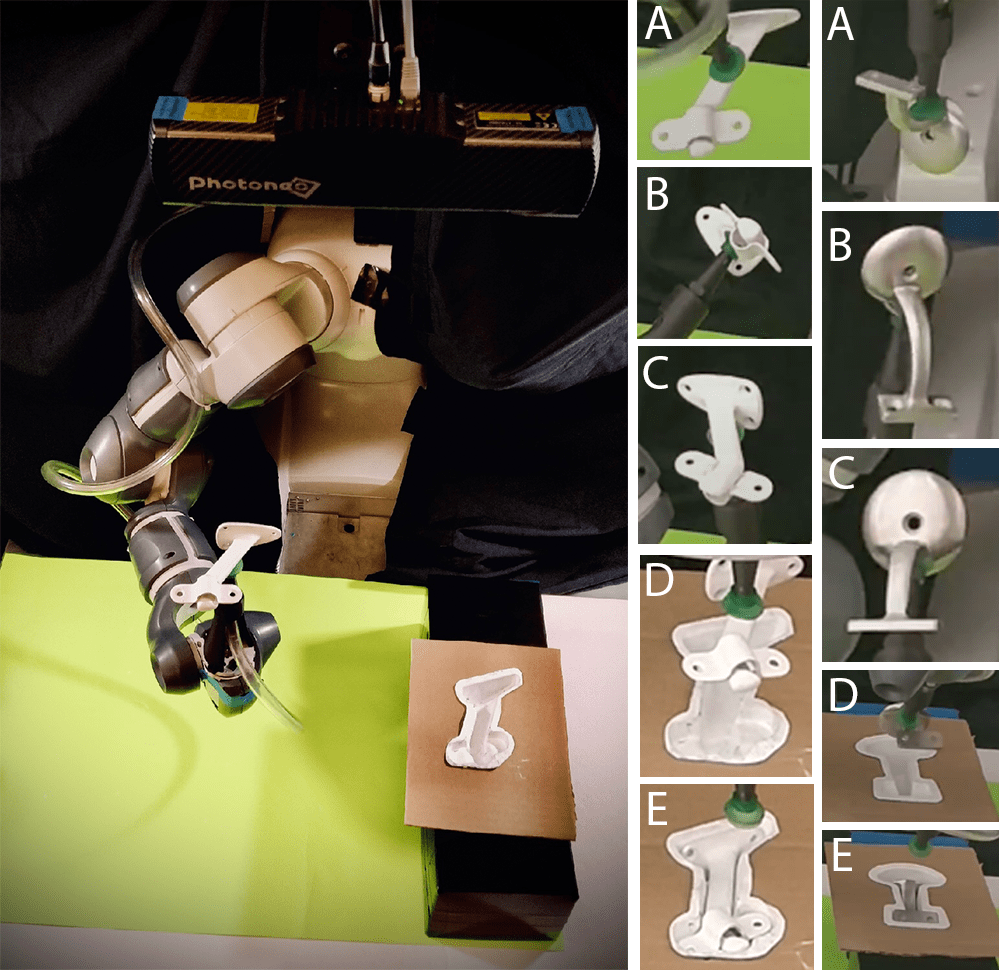
\includegraphics[width=0.48\textwidth]{figures/Fig1_Final.png}
  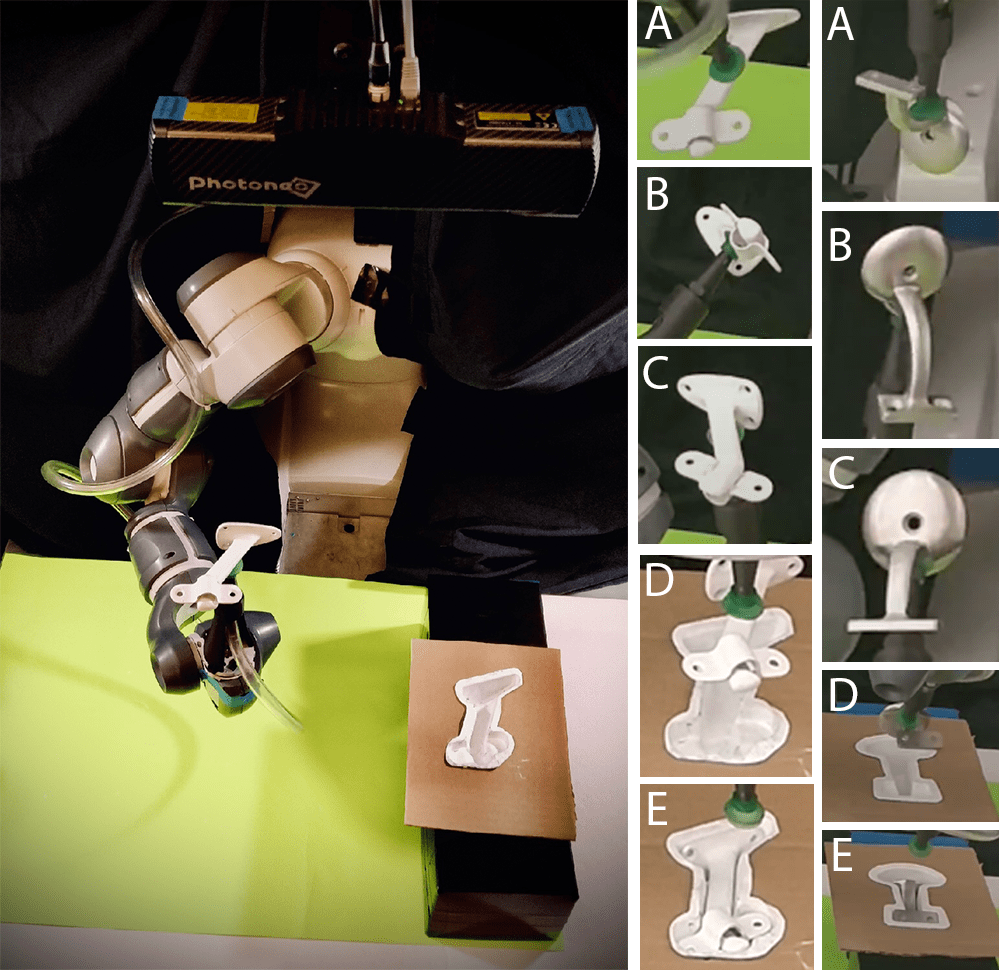
\includegraphics[width=\columnwidth,trim=0 0 187 0, clip]{figures/Fig1_Final.png}
  \caption{Physical experiments using the ABB YuMi and a Photoneo depth camera. (Left) A suction gripper holds the handrail bracket, an object unseen during training time,
  %from the top in a pose unsuitable for kitting. A 
  near the kitting cavity. % target is shown on the bottom right.
  Kit-Net orients the handrail bracket
  %(middle) and the ornamental handrail bracket (right) 
  for insertion into the cavity through 5 steps. A) Starting state. B) Rotate the object by 180\degree~to face the 3D camera and minimize occlusion from the gripper. C) Iteratively orient the object into a goal configuration. %using depth images of the kitting cavity
  D) Rotate by 180 degrees and align centroids of the object and cavity to prepare for insertion. E) Insert and release.}
  \label{fig:splash}
\end{figure}

Given a 3D CAD model of the object to be inserted and the desired object pose, one approach is to directly estimate the object pose and the transformation to the desired pose~\cite{ChoyDeepGlobal, xiang2017posecnn}. However, CAD models may not be available for all objects to be kitted and are time consuming to create for every object, motivating an algorithm that can kit previously unseen objects without requiring such models. Prior work has considered kitting objects without models, 
but has focused on $SE(2)$ transforms (1D rotation and 2D translation) for extruded 2D polygonal objects~\cite{Zakka2020Form2FitLS,zeng2020transporter}. 
% In contrast, we aim to estimate 3D rotations for previously unseen objects such that they can be matched to and inserted into a novel cavity.

% However, achieving a desired orientation often requires implicit knowledge of the object's current and desired orientation. Prior work on estimating object orientation has primarily focused on purely geometric algorithms or explicit pose estimation from sensed visual data \AB{cite} These approaches have made it possible for robots to accomplish a variety of complex manipulation tasks~\AB{cite}, but require knowledge of object geometry or do not generalize well to unseen objects~\AB{cite}.

We formalize the problem of rotating and translating a novel 3D object to insert it into a novel kitting cavity and present Kit-Net,
%an algorithm [replaced -KG 3/18]
a framework for inserting previously unseen 3D objects with unknown geometry into a novel target cavity given depth images of the object in its current orientation and a depth image of either a flipped (convex) or standard (concave) target cavity. Kit-Net extends prior work from~\citet{CASE_Orienting}, which used simulation and self-supervision to train a deep neural network to directly estimate 3D transformations between the two depth images. Given the trained deep neural network, a depth image of a previously unseen insertion cavity, and a depth image of a previously unseen object, Kit-Net iteratively estimates the $SE(3)$ transform to reorient and insert the object, without requiring detailed knowledge of its geometry. Kit-Net improves on prior work by (a) introducing dataset augmentations that make the controller more robust, (b) using a suction cup gripper to minimize object occlusion during rotation, (c) incorporating 3D translations, and (d) applying the resulting controller to kit novel objects into novel cavities on a physical robot. We evaluate Kit-Net both in simulation and in physical experiments on an ABB YuMi robot with a suction gripper and overhead depth camera. Experiments in simulation suggest that Kit-Net can orient objects to have a 98.9,\% average intersection volume between the object mesh and that of the target cavity. Physical experiments with 3 industrial objects and cavities suggest that Kit-Net can kit objects at a 63\,\% success rate from a diverse set of initial orientations. %(\todo{YY} seconds).

% We implement the algorithm on an ABB YuMi robot fitted with a suction gripper, using a top-down depth camera to provide the inputs to the algorithm.  In experiments with 4 objects of varying geometries and starting in a variety of different orientations, we find that the algorithm kits successfully \todo{XX}~\%, suggesting that the proposed method would be useful for automating kitting process.  Additionally, improving upon prior work, in experiments the algorithm computes a correct orientation in \todo{YY} steps (\todo{ZZ} seconds), suggesting that it the algorithm may be practical for speeding up kitting processes.

% Contributions:
This paper makes the following contributions:
\begin{enumerate}%[label=(\arabic*)]
\item Formulating the problem of iteratively kitting a novel 3D object into a novel 3D cavity.
\item Kit-Net: a self-supervised deep-learning framework for this problem 
\item Simulation experiments suggesting that Kit-Net can reliably orient novel objects for insertion into prismatic cavities. %, significantly improving over baseline 2D rotation methods~\cite{Zakka2020Form2FitLS,zeng2020transporter}.
\item Physical experiments suggesting that Kit-Net can significantly increase the success rate of 3D kitting into conformal 3D cavities from 18\,\% to 63\,\% over a baseline inspired by Form2Fit~\cite{Zakka2020Form2FitLS} which only considers 2D transformations when kitting. %~\cite{Zakka2020Form2FitLS,zeng2020transporter}.
\end{enumerate}
% \begin{enumerate}%[label=(\arabic*)]
% \item An algorithm to transfer the self-supervised network and controller from \citet{CASE_Orienting} to use in physical experiments for insertion into cavities.
% \item Simulation experiments suggesting that the controller can reliably \todo{}
% % orient 22 novel objects by up to 30\degree~with a median angle error of 1.47\degree~over 100 random initial/desired orientations per object.
% \item Physical experiments suggesting that the proposed controller can \todo{}
% % reorient 5 novel objects by up to 30\degree~with a median angle error of 4.2\degree~over 10 random initial/desired orientations per object.
% \end{enumerate}

% \todo{Notes from Mar 11, 2021: Additional contributions: (1) centroid,  (2) training is different (x,y) + z differences, different croppings, (3) earlier had grippers, now has suction, grippers had different occlusion problems.

% "Extended prior work in the following ways: new training set designed for this problem setting.  Robust to translation and and different kinds of occlusions."

% Tuned to a specific gripper, made it work in real better.  Practical application.

% "Formalizing the problem of kitting novel objects into cavities."

% Another contribution: real baseline comparison.
% }

\input{includes/fig1}



\section{Related Work}
\label{sec:related-work}
% Classical Methods
%Reorienting objects is an important subtask in a variety of domains, such as manufacturing, packing, and assembly.
There has been significant prior work on reorienting objects using geometric algorithms. \citet{goldberg1993orienting} proposes a geometric algorithm that orients polygonal parts with known geometry without requiring sensors. \citet{akella-orienting-uncertainty} extend the work of Goldberg with sensor-based and sensor-less algorithms for orienting objects with known geometry and shape variation. \citet{kumbla2018enabling} propose a method for estimating object pose via computer vision and then reorient the object using active probing. \citet{grasp-gaits} optimize robot finger motions to reorient a known convex object while maintaining grasp stability. In contrast to the above works, which require prior knowledge of object geometry, Kit-Net can reorient objects without 3D object models.
% Traditional Pose Estimation
% \SD{Copied from CASE: Another approach to reorienting objects explored by prior work uses statistical methods for pose estimation. The goal in this approach is to estimate the 6-DOF (translation + rotation) pose of an object with known geometry subject to uncertainty in sensing and occlusions. If 6-DOF poses can reliably be estimated, then re-orientation plans can be computed using the difference between the pose of the object in its initial orientation and its goal orientation. % and simply computing the required rotation. 
% \citet{hodan2018bop} provides eight datasets to train and test pose estimation algorithms and a consistent benchmark that works well for evaluating various methods on symmetric and partially occluded objects. \citet{prokudin2018deep, kingma2013auto} introduce a variational-auto-encoder-based probabilistic model for pose estimation. \citet{xiang2017posecnn} use semantic labeling and bounding-box prediction as surrogate tasks to perform pose estimation via quaternion regression with a new symmetry-invariant loss function.  \citet{Li2019DeepIMDI} builds on prior work by using PoseCNN~\citet{xiang2017posecnn} to provide an initial pose estimate and then iteratively refines it by matching the image rendered based on the pose estimate and the observed image of the object. 
% \citet{Do2018Deep6DPoseR6} use Mask-RCNN to perform instance segmentation and then finds a Lie algebra representation of the 6D pose of each object in a given image.
% \citet{tian2020robust} learn to predict the rotation of symmetric objects by learning directly from their RGB-D features, improve upon Shape-Match Loss of \citet{xiang2017posecnn}, and include an uncertainty on the rotation prediction. 
% \citet{peretroukhin2020smooth} proposes a novel representation of $SO(3)$ which incorporates the belief over the predicted rotation, making the learned model robust to unseen objects and scenes. 
% \citet{hagelskjaer2019using} uses spatial reasoning and workcell constraints to accurately estimate poses. \citet{deng2019self} improve upon object segmentation and pose estimation with a self-supervised method of collecting training data from real images using an RGBD camera mounted onto the hand of a robot manipulator.
% In contrast to these works, we propose a method that does not require prior knowledge of object geometry and can generalize to objects outside of those seen during training. }

% % Pose Estimation of unseen objects
% \SD{Copied from CASE: Some recent work explores pose estimation for objects unseen during training. \citet{corona2018pose} predict the pose of objects unseen at training time, but require a 3D model to adjust for ambiguities due to symmetry. \citet{Xiao2019PoseFS} trains a pose-estimation network that is conditioned on a test image and 3D object model, making it possible to predict the pose of arbitrary objects in varied visual environments if 3D models of the objects are available. These works can generalize to unseen objects, but still require 3D object models. \citet{park2019latentfusion} relax this assumption by estimating a 3D geometric model by learning a 3D object representation that enforces consistency across multiple views. Then, this estimated 3D object model can be rendered as a depth image of the object in a desired pose. This enables generalization to objects with unknown geometry, but requires that multiple views of each object are available at test time. 
% \citet{wang20196-pack} extract 3D keypoints from RGBD images of unseen objects for real-time pose tracking, but require that test objects be relatively similar to those seen in training.}

% Delta pose
\citet{delta-pose-est}, \citet{latent-3d-keypoints}, \citet{Wen2020se3TrackNetD6}, and \citet{CASE_Orienting} use data-driven approaches to estimate the relative pose difference between images of an object in different configurations.  
\citet{delta-pose-est} use a Siamese network to estimate the relative pose between two cameras given an RGB image from each camera. \citet{latent-3d-keypoints} propose KeypointNet, a deep learning approach that learns 3D keypoints by estimating the relative pose between two different RGB images of an object of unknown geometry, but known category. 
\citet{Wen2020se3TrackNetD6} considers an object tracking task by estimating a change in pose between an RGBD image of the object at the current timestep and a rendering of the object at the previous timestep, but require a known 3D object model. We use the network architecture from \citet{Wen2020se3TrackNetD6} to train Kit-Net, and extend the self-supervised training method and controller from \citet{CASE_Orienting} to kit novel objects into previously unseen cavities. We find that by extending~\citet{CASE_Orienting} to be more robust to object translations and using a suction gripper to reduce occlusions, Kit-Net is able to learn more accurate reorientation controllers.

There has also been significant interest in leveraging ideas in pose estimation for core tasks in industrial automation.
\citet{Litvak2019LearningPE} leverage CAD models and assemble gear like mechanisms using depth images taken from a camera on a robotic arm's end effector. \citet{Stevic2020LearningTA} estimate a goal object's pose to perform a shape assembly task involving inserting objects which conform to a specific shape template into a prismatic cavity. \citet{Zachares2021InterpretingCI} combines vision and tactile
sensorimotor traces for an object fitting task involving known holes and object types.
\citet{Huang2020Generative3P} consider the problem of assembling a 3D shape composed of several different parts. This method assumes known part geometry and develops an algorithm to generate the 6-DOF poses that will rearrange the parts to assemble the desired 3D shape. In contrast to the above work, we focus on the problem of designing a controller which can reorient and place a novel object within a previously unseen cavity for industrial kitting tasks. 

Object kitting has also seen recent interest from the robotics community. \citet{Zakka2020Form2FitLS} introduce Form2Fit, an algorithm which learns $SE(2)$ transforms to perform pick-and-place for kitting planar objects. In contrast, we consider 6DOF transforms of 3D objects.
\citet{zeng2020transporter} propose a network for selecting suction grasps and grasp-conditioned placement, which can generalize to multiple robotic manipulation tasks, including pick-and-place for novel flat objects. \citeauthor{zeng2020transporter} focuses on $SE(2)$ rotations and translations for pick-and-place tasks involving novel flat, 2D extruded objects. \citeauthor{zeng2020transporter} also presents an algorithm for $SE(3)$ pick-and-place tasks, but only evaluate the algorithm on 2D extruded objects. In contrast, we use Kit-Net to kit novel 3D objects with a wide range of complex geometries.
\section{Problem Statement}
\label{sec:problem-statement}
Let $T^s \in SE(3)$ be the initial 6D pose of a unknown 3D rigid object $O$ in the world coordinate frame, consisting of a rotation $R^s \in SO(3)$ and a translation $t^s \in \mathbb{R}^3$. Given $O$ with starting pose $T^s$ and a kitting cavity $K$, let $\mathcal{G} \subset SE(3)$ be the set of goal 6-DOF poses of object $O$ that result in successful kitting. The goal is to orient object $O$ to $T^g \in \mathcal{G}$, where $T^g$ consists of rotation $R^g$ and translation $t^g$. Figure~\ref{fig:mug-cavity-2} shows a simulated example where a 3D object $O$ is successfully kitted into a concave cavity $K$.
% \MD{Note about range of rotations that cause the object to kit correctly? This is implied by G but not stated explicitly anywhere. I think we need to formalize this a bit more.} \SD{We wanted some sim trials on object cavity pairs for this, but we don't have time to formalize that by March 15 because creating the cavities is pretty tough, and then we would have to setup the pybullet environment}.

\subsection{Assumptions}
\label{subsec:formulation}
We assume access to depth images of a rigid object $O$ and a kitting cavity $K$. The cavity image may be taken with the cavity either in its standard, concave orientation (i.e., open to object insertion), or flipped, convex orientation (i.e., mirroring the shape of the object to be inserted).
% We also assume that the rotation angle between $R^s$ and $R^g$ is at most 30\degree \SD{Can we say 45 degrees or 60 degrees? It can be 60 degrees away from a correct orientation, but still be 30 degrees from the set of correct orientations}. 
We also assume that orienting $O$ to a pose in $T^g \in G$ and releasing the gripper results in a successful kitting action.

\begin{figure}[t]
  \centering
  \vspace{8pt}
  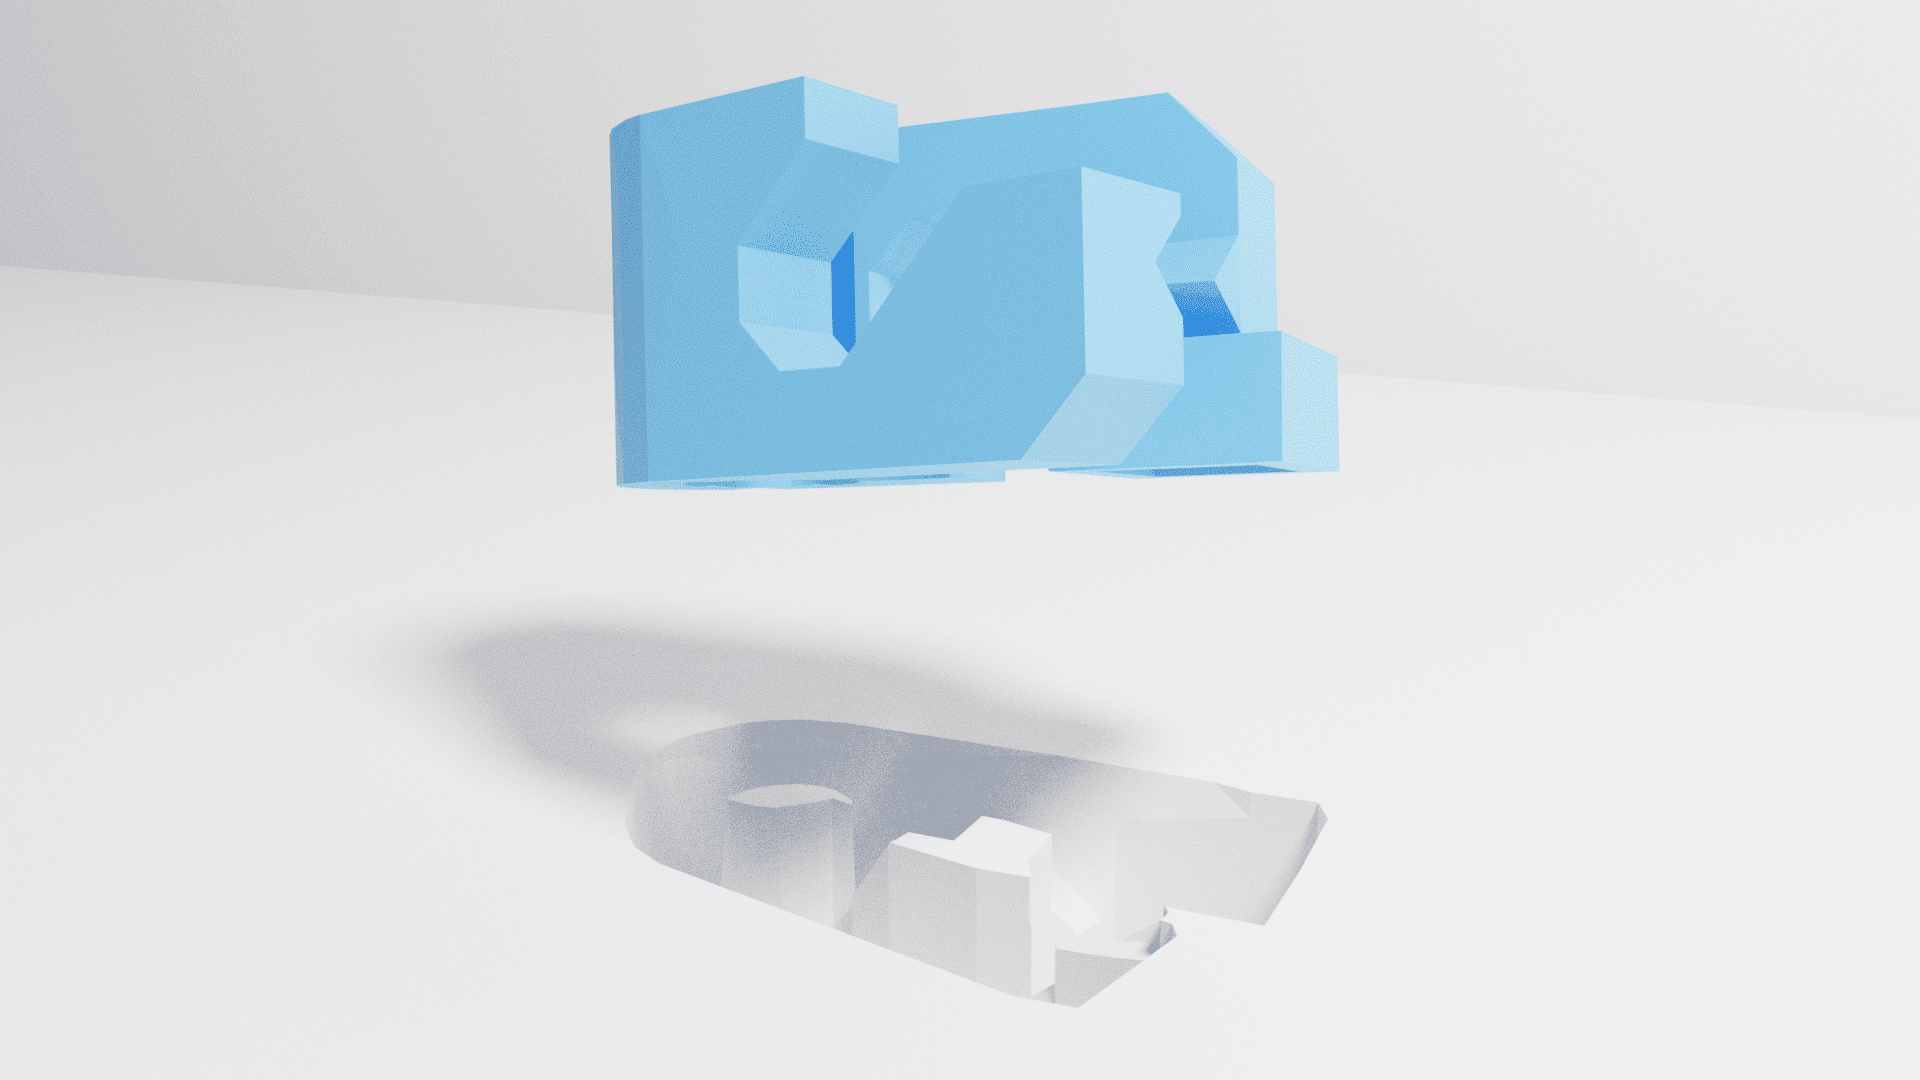
\includegraphics[width=121pt,trim=440 0 440 0, clip]{figures/bar_clamp_impression_2.png}\hfill%
  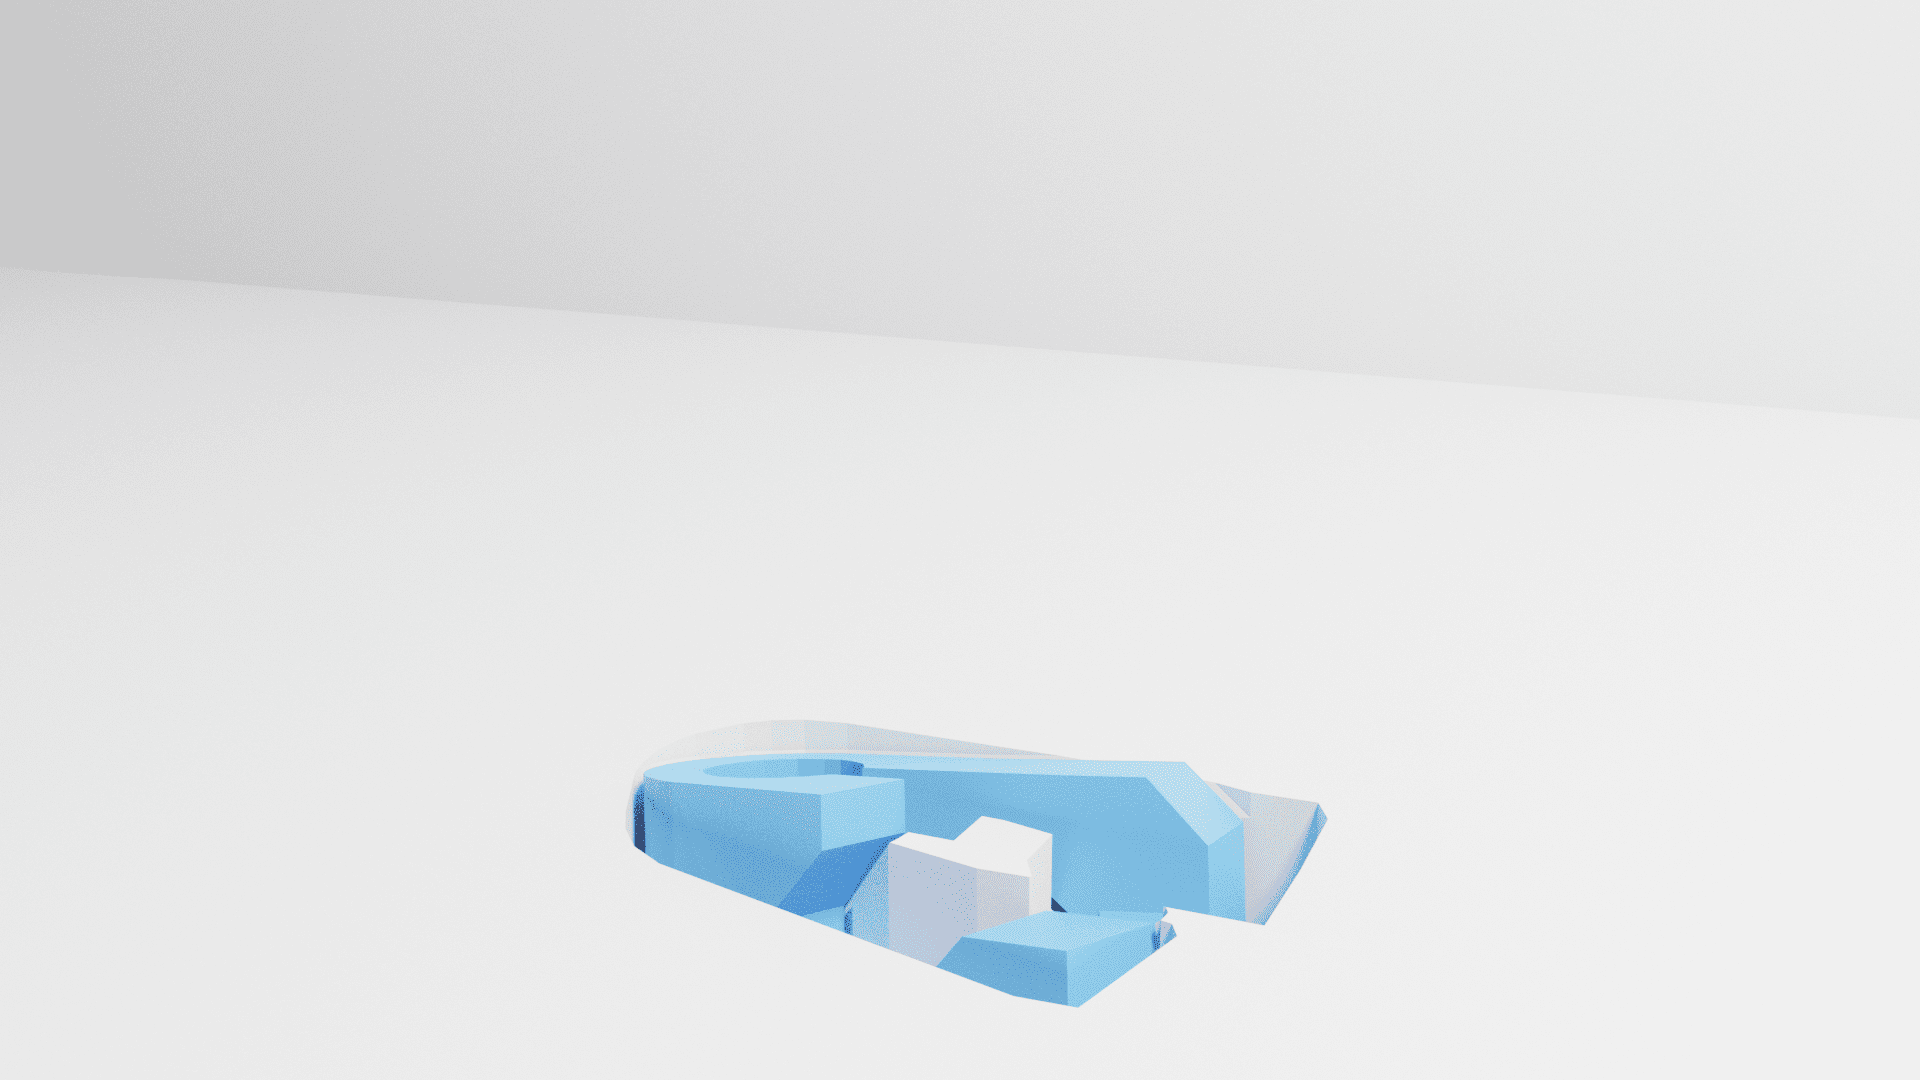
\includegraphics[width=121pt,trim=440 0 440 0, clip]{figures/bar_clamp_impression_4.png}
  \caption{\textbf{Successful Kitting: }Visualization of successfully kitting a 3D object into a concave cavity.}
  %\caption{\textbf{Generating Negative Goal Images: }Example an object (left) in a specific configuration $T^g$ and its complementary cavity created in simulation with Blender. We use the fatten operation to create a cavity with some slack for insertion (right). 
%   This cavity requires orienting the object to $\mathcal{G}$, a range of poses close to $T^g$ in order to be oriented.
  %}
  \label{fig:mug-cavity-2}
\end{figure}
\subsection{Input}
\label{subsec:input}
Let $I^s \in \mathbb{R}^{H \times W}$ be a depth image observation of the object in initial pose $T^s$, and
$I^k \in \mathbb{R}^{H \times W}$ be the depth image observation of a kitting cavity, $K$. See Figure~\ref{fig:clamshell-cavities} for physical examples of objects and kitting cavities.

\subsection{Output}
\label{subsec:output}
%As shown in Fig.~\ref{fig:splash} and Fig.~\ref{fig:mug-cavity-2},
The goal is to successfully kit an unknown 3D object $O$ into a novel 3D cavity $K$ (Fig.~\ref{fig:splash}, Fig.~\ref{fig:mug-cavity-2}). Thus, we aim to transform the initial pose $T^s$ into a goal pose that fits into the cavity (i.e., $T^g \in \mathcal{G}$). For objects with symmetries, the objective is to estimate and orient objects relative to a (symmetric) orientation that results in successful insertion into the cavity K.

% \subsection{Background}
% We use unit quaternions to represent rotations.
% A quaternion $q = q_r + q_i i + q_j j + q_k k$ is an extension of complex numbers with a real component $q_r$ and 3 scaled fundamental imaginary units $i$, $j$, and $k$.
% We represent $q$ using the convention of a vector $\begin{bmatrix} q_r & q_i & q_j & q_k \end{bmatrix}^T$. 
% A \emph{unit} quaternion has the property that $\lVert q \rVert^2 = q_r^2 + q_i^2 + q_j^2 + q_k^2 = 1$, and can represent a rotation with properties we make use of in this work:
% \begin{description}[left=0pt]
%     \item[Normalization] A unnormalized or non-unit quaternion $\tilde{q}$ can be converted to a unit quaternion by dividing by its norm $\tilde{q} / \lVert \tilde{q} \rVert_2$
%     \item[Angle difference] The angle of rotation $\theta$ between two quaternions $q_0$ and $q_1$ is $2\cos^{-1} \lvert \langle q_0, q_1 \rangle \rvert$
%     \item[Rotation difference] The quaternion rotation between two quaternions is $q_{\mathrm{diff}} = q_0 q_1^{-1}$, where $q_1^{-1}$ is the conjugate (negated imaginary components) of $q_1$
%     \item[Slerp] The spherical linear interpolation or \emph{slerp} between rotations $q_0$ and $q_1$ by a scalar $t \in [0,1]$ is  $\Slerp(q_0, q_1, t) = (q_0 \sin (1-t)\theta + q_1 \sin t\theta) / \sin \theta$, where $\theta$ is the angle between the two rotations~\cite{shoemake}.
%     \item[Angle of rotation] The angle of rotation of a quaternion is defined by $\quattoangle(q) = 2 \cos^{-1} q_r$
%     \item[Axis of rotation] The axis of rotation of a quaternion is $\begin{bmatrix} q_i & q_j & q_k \end{bmatrix} / \sqrt{1 - q_r^2}$
%     \item[Double Coverage] Quaternions double cover $SO(3)$, in that $q$ and $-q$ represent the same rotation.
% \end{description}

% \section{Method}
\section{Kit-Net Framework}
\label{sec:method}
%\JI{Proposal: include summary of \cite{CASE_Orienting} in first subsection, then describe extensions in second subsection.} \SD{Done?}
We present Kit-Net, a framework that first reorients the object into a pose that can be successful kit in a desired cavity, and then translates and inserts the object into the cavity. We do this by learning to estimate ${_s}T^g \in SO(3)$, a relative transformation consisting of rotation ${_s}R^g$ and translation ${_s}\hat{t}^g$, which transforms the object from $T^s$ to $T^g$ for some $T^g \in \mathcal{G}$. The overall approach is to (1) compute an estimate of ${_s}R^g$, denoted ${_s}\hat{R}^g$, given only image observations $I^s$ and $I^k$, (2) iteratively reorient the object according to  ${_s}\hat{R}^g$ until $\hat{R}^g \in \mathcal{G}$, and (3) translate the object by ${_s}\hat{t}^g$, an estimate of the translation between the start and goal object translations, such that it lies in the kitting cavity.

We first discuss preliminaries (Section~\ref{subsec:prelims}) and then describe the key new ideas in training Kit-Net (Section~\ref{subsec:kit-net-training}) which make it possible to design a controller to rotate and translate an object to fit it in a cavity (Section~\ref{subsec:kit-net-alg}).

% \subsection{Prior Work: Aligning Quaternion Rotations in 3D}
\subsection{Preliminaries: Estimating Quaternion Rotations in 3D}
\label{subsec:prelims}
\citet{CASE_Orienting} presented a self-supervised deep-learning method to align
two 3D objects.
%an object to a goal rotation. 
The method takes two depth images as input: $I^s$, an image of the object in its current orientation $R^s$ and $I^g$, an image of the same object in its desired goal orientation $R^g$. It trains a deep neural network $f_\theta:\mathbb{R}^{H\times W},\mathbb{R}^{H\times W} \rightarrow SO(3)$
to estimate the rotation (parametrized by a quaternion) between the pair of images $(I^s, I^g)$.
% that acts on the depth image pair learns how to estimate rotations (parametrized by a quaternion) between two poses of an unknown object. 
Then, using a proportional controller, it iteratively rotates the object to minimize the estimated rotational difference. This controller applies $\eta{_s}\hat{R}^g$ until
% there have been $50$ iterations or
the network predicts that the current object rotation $R^s$ is within $\delta = 0.5\degree$~of $R^g$, or until the controller reaches an iteration limit. The tunable constant $\eta$ is the Spherical-Linear intERPolation (slerp) factor describing the proportion of $\hat{R}^g$ that the controller will apply to $O$. \citeauthor{CASE_Orienting} use a small slerp value of $\eta=0.2$ and a maximum iteration limit of 50 rotations.

For training,~\citeauthor{CASE_Orienting} generate a dataset consisting 200 pairs of synthetic depth images for each of the 698 training objects with random relative rotations, for a total of 139,600 pairs. To account for parallax effects, each pair of images were generated from a fixed translation relative to the camera.
\citeauthor{CASE_Orienting} propose three loss functions to train $f_\theta$: a cosine loss, a symmetry-resilient loss, and a hybrid of the two, with the hybrid loss outperforming the first two. Note that \citeauthor{CASE_Orienting} do not consider cavity insertion tasks, which is complicated by the need to reason about the translations and required alignment with a cavity. 
%, which may differ significantly in geometry from the object being inserted.  [<- "future work" -KG]

Kit-Net improves on \citeauthor{CASE_Orienting} by (1) introducing dataset augmentations to make the controller more robust, (2) using a suction cup gripper to minimize object occlusion during rotation, and (3) incorporating 3D translations into the controller to enable kitting. We discuss these contributions in the following sections.

\subsection{Kit-Net Dataset Generation, Augmentation, and Training}
\label{subsec:kit-net-training}
% \JI{TODO: we need to update this section to make fewer repeated references to [5].  If the previous section is sufficiently filled in, then we can also focus on describing the updates from the previous section.} \SD{Done?}
Kit-Net %extends \citet{CASE_Orienting} to 
trains a neural network $f_\theta$ with a self-supervised objective by taking as input pairs of depth images $(I^s, I^g)$ and estimating ${_s}\hat{R}^g$ from image pair $(I^s, I^g)$. As in \citeauthor{CASE_Orienting}, $f_\theta$ encodes each depth image into a length 1024 embedding, concatenates the embeddings, and passes the result through two fully connected layers to estimate a quaternion representation of the rotational difference between the object poses. 

\subsubsection{Initial Dataset Generation}
In contrast to \citeauthor{CASE_Orienting}, we are interested in kitting, rather than just reorienting an object in the robot gripper. Thus, in this paper we focus on two types of kitting cavities: prismatic cavities (Fig.~\ref{fig:prism-task}) and conformal cavities (Fig.~\ref{fig:clamshell-cavities}).
We generate a separate dataset for each type of cavity and train a separate network for each dataset. 
To generate both datasets, we use the set of 698 meshes from \citet{mahler2019learning}. For each mesh, we generate 512 depth image pairs, for a total of 357,376 pairs. To do this we first generate a pair of rotations $(R^s, R^g)$, where $R^s$ is generated by applying one rotation sampled uniformly at random from $SO(3)$ to $O$, and $R^g$ is generated by applying a random rotation with rotation angle less than 30 degrees onto $R^s$. To generate the conformal cavity dataset, we then obtain a pair of depth images $(I^s, I^g)$ by rendering the object in rotations $R^s$ and $R^g$ from an overhead view. The pair is labeled with the ground truth rotation difference between the images. To generate the prismatic cavity dataset we follow the same process as above, except we fit and render a prismatic box around the rotated object (Fig.~\ref{fig:prism-task-eval-objects}) and render the depth image pairs (Fig.~\ref{fig:prism-task}). This process results in two datasets, each containing 357,376 total labeled image pairs $(I^s, I^g)$ with ground truth rotation labels ${_s}R^g$. 

\subsubsection{Data Augmentation}
We found that simply training a network directly on the datasets described above results in poor generalization to depth images from the physical system, which contain sensor noise, object occlusions from both the object itself and the arm or gripper, and 3D object translations within the image. To address these three points, we introduce a set of dataset augmentations to ease network transfer from simulated to real depth images. 
%To increase network robustness to sensor noise and occlusions, [omit as we haven't quantified this increase -KG 3/18]
To simulate noise and occlusion in training, we randomly zero out 1\,\% of the pixels in each depth image and add rectangular cuts of width 30\,\% of zero pixels to the image, respectively.
%To increase robustness to object translations, [omit as we haven't quantified this increase -KG 3/18]
To simulate translations in training,
we translate the object across a range of 10\,cm in the $x$, $y$, and $z$ axes with respect to the camera in the simulated images. We also crop the images at sizes from 5\,\% to 25\,\% greater than the object size with center points offset from the object's centroid by 5 pixels to simulate
%These translations allow the trained network to be robust to
$I^s, I^g$ pairs generated from objects and cavities outside the direct overhead view for the kitting task. 

% consider a wide range of object translations \KG{$\leftarrow$ Details!!} within the image and render and crop images with varying sizes and centers \KG{$\leftarrow$ Details!!} to make the network more robust to images from the physical system \KG{$\leftarrow$ Details!!}. Specifically, we augment the dataset images with randomly generated zero pixels and rectangular cuts 
% \SD{I have not explicitly tried performance without this, but I have observed self-occlusion on the real images that I believe the random cuts help make the network robust to} 
% to make the network more robust to occlusions \KG{why if suction grasps?} and sensor noise present in depth images taken from a real depth camera. We also render objects in a wider range \KG{\#s} of $x$, $y$, and $z$ coordinates, in an effort to allow the network to be robust to $I^s, I^g$ pairs generated from objects and cavities outside the direct overhead view for the kitting task. 

\subsubsection{Training} We adopt the network architecture from \citet{Wen2020se3TrackNetD6}, as it is designed to be trained in simulation and demonstrates state-of-the-art performance on object tracking~\cite{DengPoseRBPF} by regressing the relative pose between two images. We use the hybrid quaternion loss proposed by \citet{CASE_Orienting}. The network is trained with the Adam optimizer with learning rate 0.002, decaying by a factor of 0.9 every 5 epochs with an L2 regularization penalty of $10^{-9}$.

\subsection{Kit-Net Suction Gripper}
Kit-Net uses an industrial unicontact suction gripper from \citet{mahler2017suction} to grasp the object for kitting. In contrast, \citeauthor{CASE_Orienting} used a parallel jaw gripper. We find the suction gripper to be better suited for kitting because it reduces gripper occlusions % when the object is in hand  [removed -KG 3/18]
and enables the robot to position the object directly inside the kitting cavity.

\subsection{Kit-Net Controller} \label{subsec:kit-net-alg}
The Kit-Net controller consists of two stages: rotation and translation.

\subsubsection{Rotation}
Kit-Net first re-orients an object using the depth image of the current object pose $I^s$ and a depth image of the goal cavity pose $I^g$. In preliminary experiments, we found the rotation parameters used by \citet{CASE_Orienting} (Section~\ref{subsec:prelims}) to be overly conservative. Thus, to speed up the alignment process, we use a larger slerp factor of $\eta=0.8$. If the network predicts a rotation difference of less than $\delta=5\degree$, then we assume that the object is close enough to the required pose for kitting into the cavity and terminate the rotation controller. Because of the larger slerp value, Kit-Net is able to quickly reorient the object, thus we terminate the rotation controller after a maximum of 8 sequential rotations (8 iterations). 

\subsubsection{Translation}
Once the rotational alignment is computed, Kit-Net computes a 2D translation to move the object directly over the target cavity, and then lowers the object and releases it into the cavity. To calculate the 2D translation, we perform centroid matching between the final depth image $I^s$ of the object after rotation and the depth image of the cavity $I^g$.
% to find ${_s}\hat{t}^g$, which we combine to determine ${_s}\hat{T}^g$.
%To compute the translation, we calculate the difference of the 2D centroid of the cropped depth images of the object from the cavity (See~\ref{fig:Kit-Net-to-cavity}).
%We found in experiments that this approach was sufficiently robust to noise and outliers in the depth images and crops to achieve high accuracy.
%We conjecture that other methods such as least squares on a small set of corresponding points could lead to higher accuracy. [<-- future work -KG]



% \subsection{Controller}
% \label{subsec:reorientation-controller}

% As predictions from the trained network empirically have errors proportional to the actual angle difference, a single rotation prediction may not reorient an object correctly.  We thus implement a proportional controller to incrementally reorient the object. This controller is defined in Algorithm~\ref{alg:controller}.
% Let $I^{(t)}$ denote an overhead image of the object at some time $t$. Given a goal image $I^g$, the controller uses $f_\theta$ to predict a rotation to align the orientation corresponding to $I^{(t)}$ ($R^t$) with that corresponding to $I^g$ ($R^g$).  In each iteration, it rotates the object in the direction of the prediction by a tunable step-size parameter $\eta \in (0,1]$, and stops once the predicted angle is small or it reaches an iteration limit. %We do this by using the learned rotation estimation network $f_\theta$ to define a proportional controller (P-controller) as follows:

% \subsection{Aligning Translation}


% \subsection{Regrasp Analysis}

% \todo{If implemented... describe what happens if the suction grasp is on the wrong side, preventing both rotational alignment and insertion.}
% \DB{Even if we just show we can detect the need for a regrasp, I think that would be nice to show. We can then say that future work could use something like the BORGES algorithm [cite] to regrasp the object in a different stable pose.}
\section{Simulation Experiments}
\label{sec:experiments}
We first discuss metrics to evaluate performance in Section~\ref{subsec:metrics}. We then introduce a baseline algorithm (Section~\ref{subsec:baseline}) with which to compare Kit-Net and present experimental results in Section~\ref{subsec:results}. In experiments, we first evaluate Kit-Net on re-orienting novel objects with unknown geometry into a target prismatic box in simulation (Section~\ref{subsubsec:prismatic}).
\subsection{Baselines}
\label{subsec:baseline}
\subsubsection{Random Baseline}
We also compare Kit-Net with a baseline that applies a randomly sampled rotation but with the correct rotation angle to evaluate how important precise reorientation is for successful kitting.

\subsubsection{2D Baseline}
To evaluate the importance of estimating 3D rotations for successful kitting, we compare Kit-Net to a baseline inspired by %Transporter Nets~\cite{zeng2020transporter} and
Form2Fit~\cite{Zakka2020Form2FitLS}, which only considers 2D rotations when orienting objects for kitting. The baseline (1) aligns the centroids of the point clouds of the object and the cavity and (2) searches over all possible $z$-axis rotations at a 1\textdegree~discretization to find the rotation that minimizes Chamfer distance between the centroid-aligned point clouds.

\subsection{Metrics}
\label{subsec:metrics}
\subsubsection{Object Eccentricity}
We categorize test objects by their \emph{eccentricity}, which provides a measure of kitting difficulty. This categorization
% is grounded in the intuition [<-- lol]
follows the intuition
that objects that are more elongated along certain dimensions than others have a smaller set of acceptable orientations in which they can be successfully kit into a cavity. Let the eccentricity $\varepsilon$ of a 3D object be $\varepsilon = A - 1$, where $A$ is the aspect ratio (ratio of longest side to shortest side) of the minimum volume bounding box of the object. This definition generalizes the 2D definition of eccentricity from \citet{GoldbergEccentricity2000} to 3D. Under this definition, a sphere has $\varepsilon = 0$, and if one axis is elongated by a factor $p$, then the resulting ellipsoid has eccentricity $p-1$. This definition is also consistent with the intuition provided earlier, as a sphere is entirely rotationally symmetric, and thus does not require any reorientation for kitting. By contrast, the ellipsoid will require reorientation to ensure that its longer side is aligned to a region with sufficient space in the cavity. Thus, we use objects with high eccentricity in evaluating both Kit-Net and the baselines, as these objects pose the greatest challenge for kitting in practice.

\subsection{Results}
\label{subsec:results}
When evaluating Kit-Net in simulation, we have access to ground-truth object and cavity geometry. Thus, we evaluate kitting performance using the following percent fit metric:
\begin{equation}\label{eq:percent-fit}
\hat{f}(I^s, I^g, \hat{{_s}T^g}) = \frac{1}{N} \sum_{i=1}^N \mathbf{1}_{(p_i \in K)},
\end{equation}
where we sample $N$ points within the object volume at configuration $\hat{{_s}R^g}R^s$ (after the target object has been rotated for insertion) and count the proportion of sampled points that also lie within cavity. This metric can be efficiently computed using ray tracing and effectively estimates how much of the object fits inside the target mesh after the predicted rotation.
%This metric takes an average of 0.2\,s to compute with ray tracing on CPU \MD{which CPU? how many trials?} \MD{time depends on num rays and object geometry right?}. 
In experiments, we use $N=10000$ sampled points to evaluate $\hat{f}$. Assuming the true percent fit metric is $f$, a 95\,\% confidence interval for $f$ is $\hat{f} \pm 1.96\sqrt{\frac{\hat{f}(1-\hat{f})}{10000}}$. For example, if $\hat{f} = 0.99$, then $f$ lies between $(0.988, 0.992)$ with 95\,\% confidence. 



%\subsection{Results}


\subsubsection{Simulated Kitting into a Prismatic Target}
\label{subsubsec:prismatic}
\begin{figure}[t]
  \vspace{8pt}
  \centering
  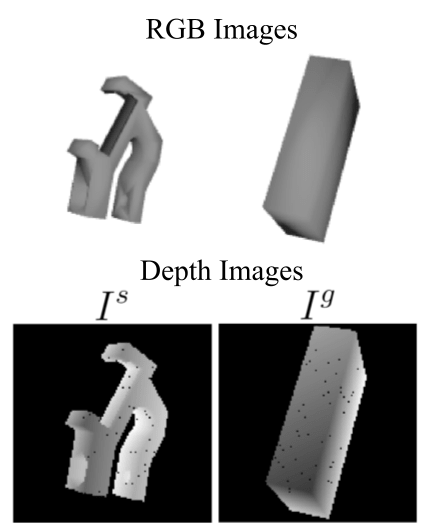
\includegraphics[width=0.8\linewidth]{figures/prismatic_example_labeled.png}
  \caption{\textbf{Endstop Holder and Target Prismatic Cavity in Simulation: } Given $I^s$, an image of an object in some configuration (top left) and $I^g$, an image of a target prismatic box to which the object must be aligned (top right), the objective is to find a 3D rotation $\hat{{_s}R^g}$ that would allow the object to fit within the box. In simulation experiments, $R^g$ is a $X$\degree~rotation from $R^s$, where $X\in (0,30)$. The image in the figure shows a 30\degree rotation, meaning the object must be rotated by 30\degree to perfectly fit it inside the prism. 3D models corresponding to $I^s$ and $I^g$ are shown in the bottom row for clarity. 
  }
  \label{fig:prism-task}
\end{figure}

We first study whether Kit-Net can orient objects into alignment with a prismatic cavity that loosely conforms to their 3D geometry in simulation. Precisely, we first generate the prismatic cavity for the target by creating a mesh with faces corresponding to its minimum volume bounding box. We then rotate both the prismatic cavity and target to random orientations within 30 degrees of each other. The objective is to apply a rotation ${_s}\hat{R}^g$ that will allow the object to fit into the cavity. An example image pair of an object and an associated prismatic cavity is shown in Figure~\ref{fig:prism-task}.

Fig.~\ref{fig:mean-percent-fit-ecc} shows the percent fit across 174 unseen test objects. We use the eccentricity $\epsilon$ of the objects to sort them into 5 bins of increasing difficulty (increasing $\epsilon$). We find that Kit-Net is able to reliably kit novel objects, significantly outperforming the 2D rotation baseline. When averaged across all eccentricities, Kit-Net achieves an average fit of 98.9\,\% compared to an average fit of 93.6\,\% for the 2D baseline and 83.1\,\% when applying a random 30\degree~quaternion. These results demonstrate the need for 3D rotations to solve complex kitting problems. Figure~\ref{fig:mean-percent-fit-ecc} demonstrates that Kit-Net is robust to highly eccentric objects which require the most precision for kitting. Kit-Net achieves an average fit of 89.9\,\% for objects with eccentricity greater than 8. The 2D rotation baseline performs especially poorly for these difficult objects and achieves an average fit of only 72.7\,\% while applying a random 30\degree~quaternion results in an average fit of just 37.4\,\%.

As described in Section~\ref{subsec:kit-net-alg}, Kit-Net iteratively orients each object using the controller until $\hat{{_s}R^g}\leq 5\degree~$ or until we hit the stopping condition of 8 rotations. Our previous results in Fig.~\ref{fig:mean-percent-fit-ecc} suggests that Kit-Net can consistently align objects within 5 controller steps.
To better visualize the ability of Kit-Net to rapidly reorient an object for kitting, we plotted the per-iteration performance of Kit-Net for 4 test objects unseen during training time with high eccentricity ($\epsilon \geq 2$).  Fig.~\ref{fig:prism-task-eval-objects} shows renderings of these objects along with outlines of the corresponding prismatic kitting cavities. Fig.~\ref{fig:percent-fit-runs} shows the average per-iteration percent fit across 100 controller rollouts of randomly sampled $(I^s,I^g)$ pairs for each object. We find that Kit-Net is able to consistently align objects with their target prismatic cavities, and achieves a median fit percentage of 99.4\,\% after only 3 successive reorientations. By contrast, the 2D baseline is not able to surpass an average fit of 90\,\% for any of the objects. The results in Fig.~\ref{fig:percent-fit-runs} validate the importance of iteratively reorienting parts and demonstrates that applying multiple iterations of the rotation output by the trained network can greatly help to reduce the error between $\hat{{_s}R^g}R^s$ and $R^g$ as compared to a single iteration. 
%DB{it would be nice to include a failure case here as well} 
% and for many objects, including the four shown in Figure~\ref{fig:prism-task-eval-objects}, Kit-Net achieves successful alignment in just 3 steps (Figure~\ref{fig:percent-fit-runs}).

\begin{figure}[t]
  \centering
  \vspace{8pt}
  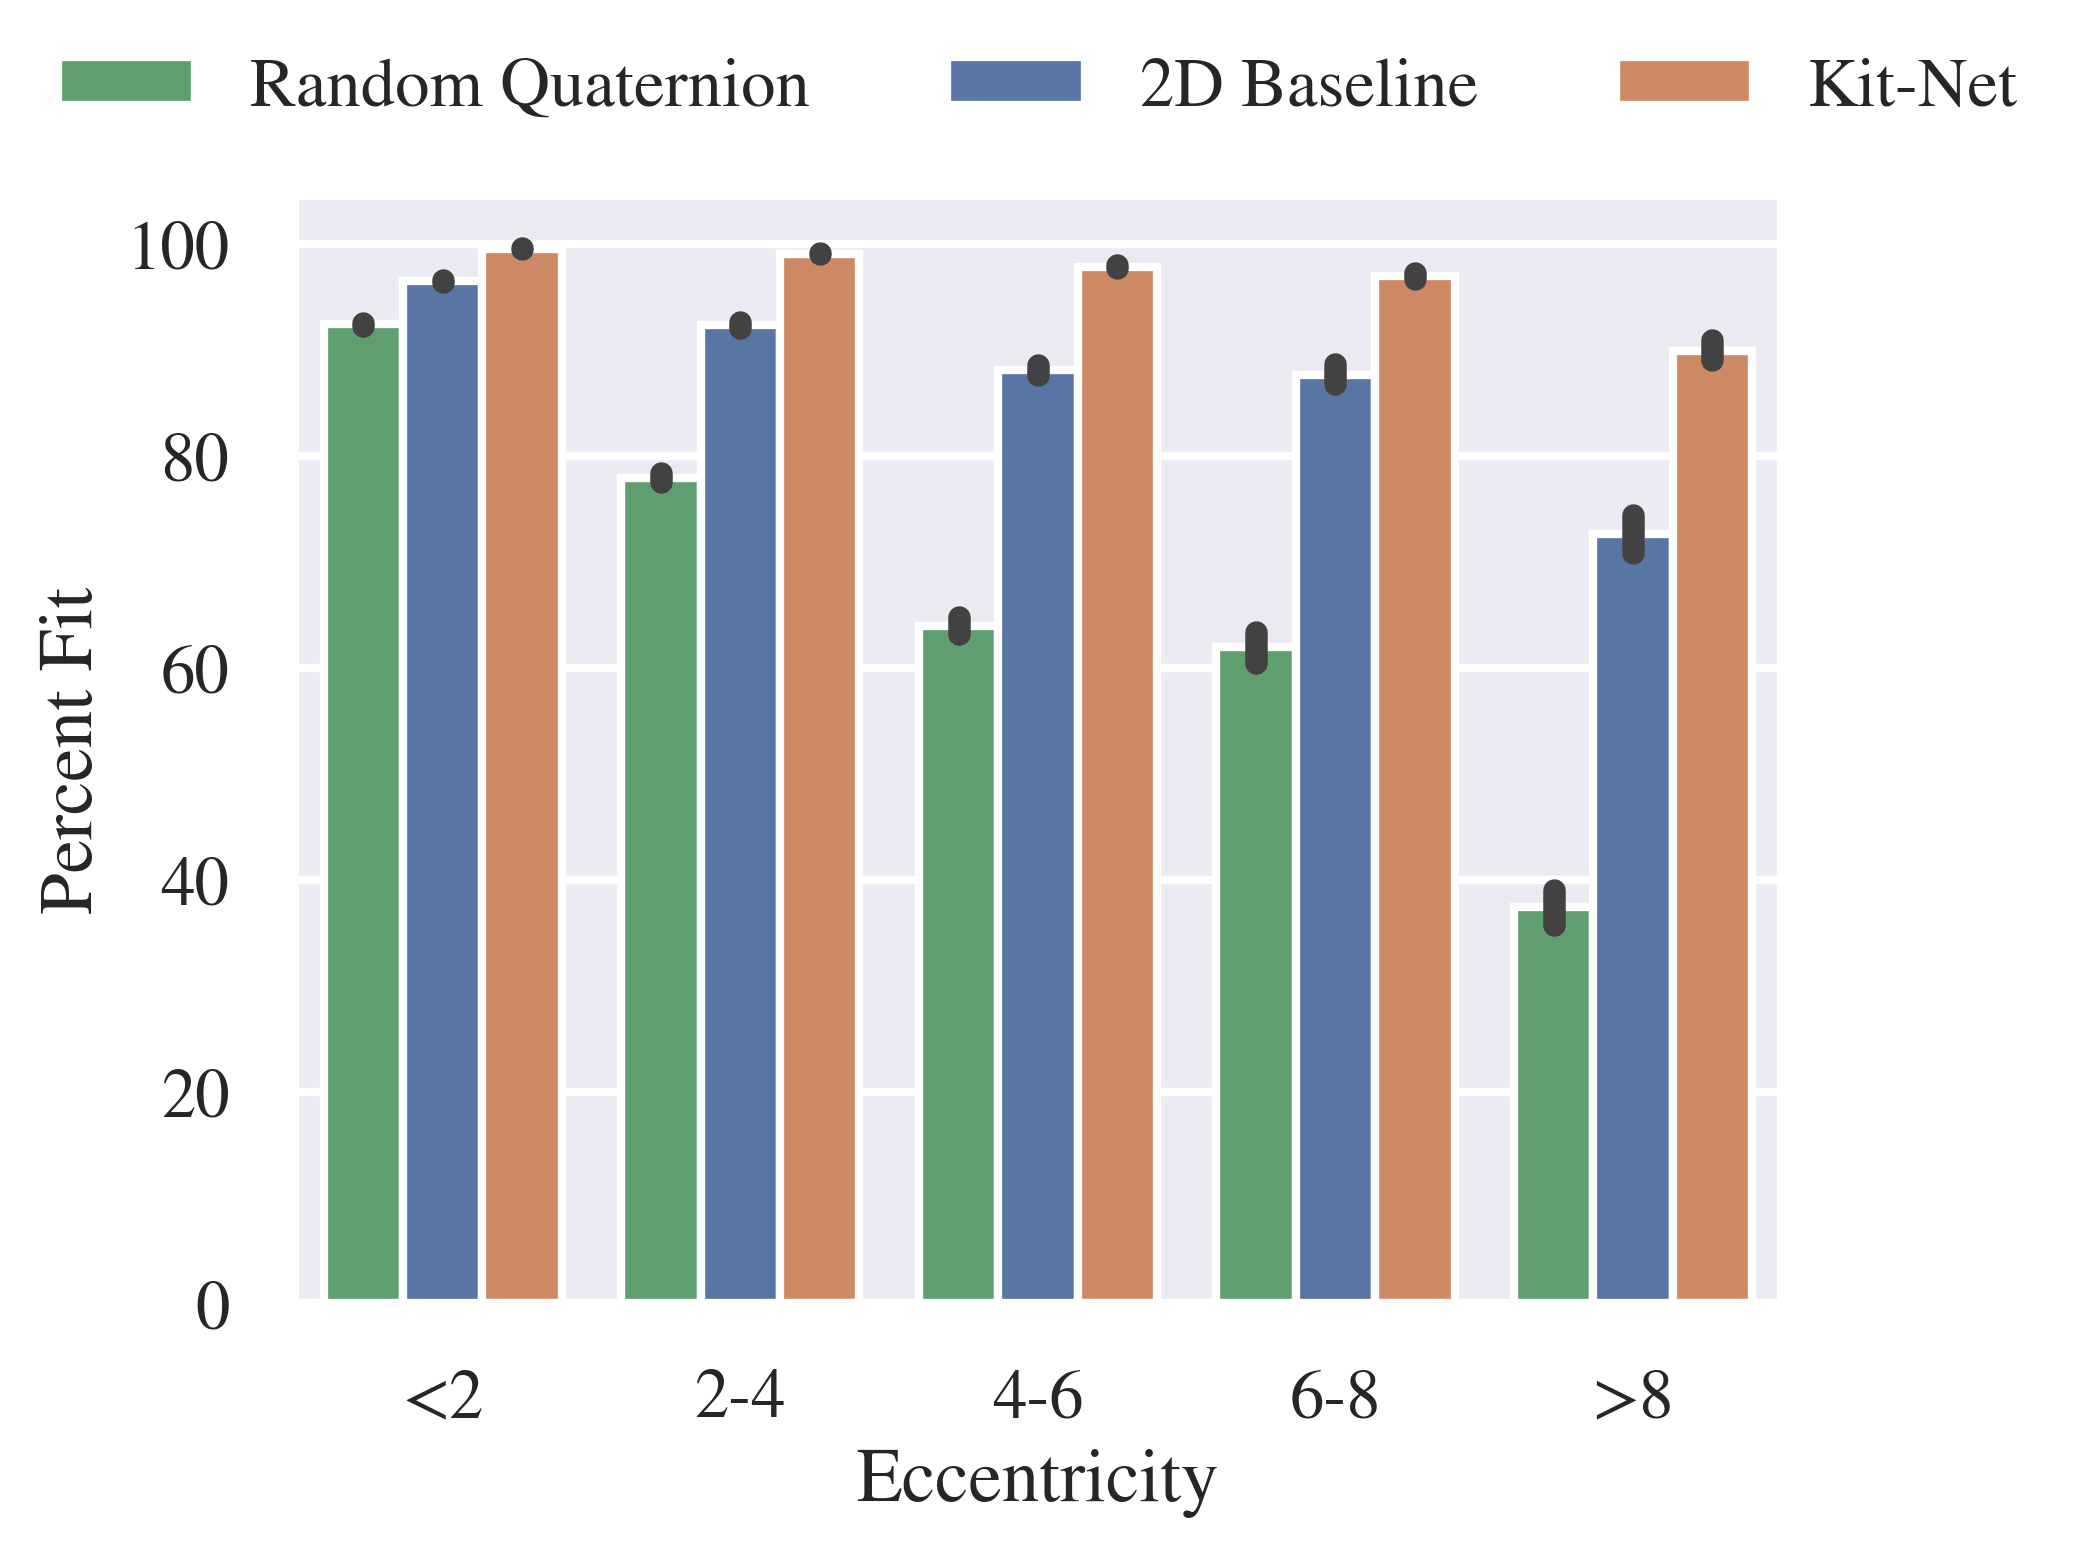
\includegraphics[width=\linewidth]{figures/percent_fit_ecc_v4.png}
  \caption{\textbf{Aligning Objects to Prismatic Cavities in Simulation: }We evaluate Kit-Nets ability to align objects with prismatic cavities under the percent fit metric introduced in Section~\ref{subsec:metrics} across 512 depth image pairs for each of 174 objects not seen during training. Given $(I^s,I^g)$, the network predicts $\hat{{_s}R^g}$ that will allow it to fit inside the cavity. We bin results by object eccentricity and observe that the mean percent fit decreases for objects of higher eccentricity. Kit-Net outperforms both the 2D and random baselines by a greater amount as object eccentricity increases.}
  \label{fig:mean-percent-fit-ecc}
\end{figure}

%  Figure~\ref{fig:percent-fit-runs} shows the progression of 16 runs of the controller on 4 randomly sampled  pairs for objects unseen in training and Figure~\ref{fig:percent-fit-hist} visualizes the distribution of fit percentages over 100 controller rollouts for each of the 4 eccentric objects visualized in Figure~\ref{fig:prism-task-eval-objects}. Results suggest that Kit-Net achieves a median final fit percentage of 99\%, suggesting that Kit-Net can effectively kit novel objects in novel prismatic cavities. \SD{Mike will add all the new Figures for eccentricity vs fit, controller rollout, controller histogram. Also baseline and then write about the figures here}

\begin{figure}[t]
  \centering % trim=left bottom right top, clip
%   \begin{tabular}{@{}c@{\enspace}c@{\enspace}c@{\enspace}c@{}}
%   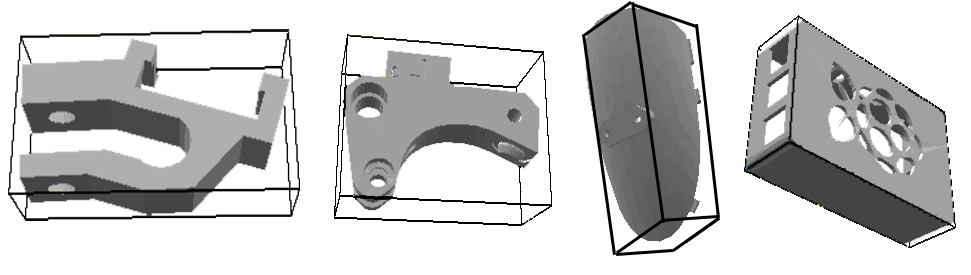
\includegraphics[height=54pt, trim=7 53 670 28, clip]{figures/Industrial Prismatic Cavity Task Objects.png} &
%   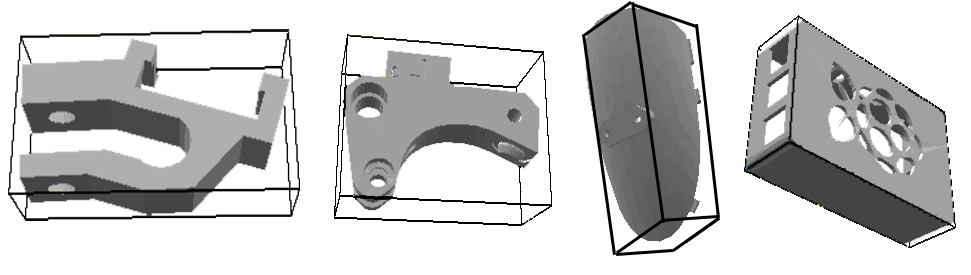
\includegraphics[height=54pt, trim=333 48 418 33, clip]{figures/Industrial Prismatic Cavity Task Objects.png} &
%   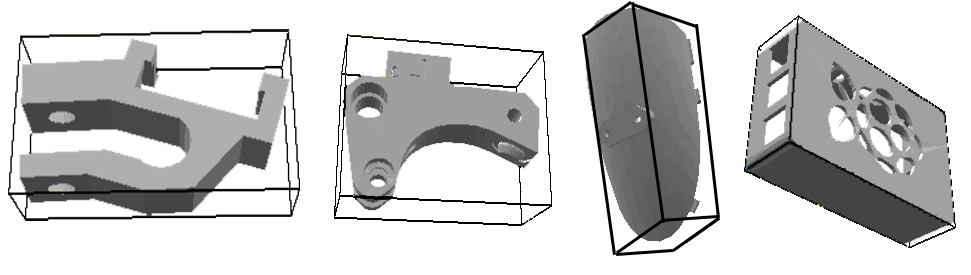
\includegraphics[height=54pt, trim=581 18 250 0, clip]{figures/Industrial Prismatic Cavity Task Objects.png} &
%   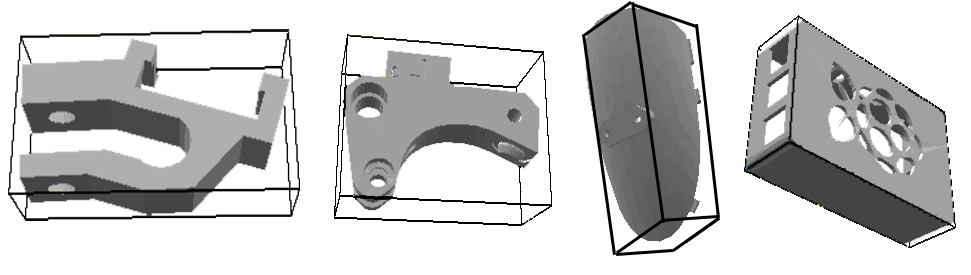
\includegraphics[height=54pt, trim=743 26 14 14, clip]{figures/Industrial Prismatic Cavity Task Objects.png} \\
%   \footnotesize Endstop holder &
%   \footnotesize Industrial part &
%   \footnotesize Shield part  &
%   \footnotesize Raspberry Pi case \\
%   \end{tabular}
  \subcaptionbox*{Industrial Part}{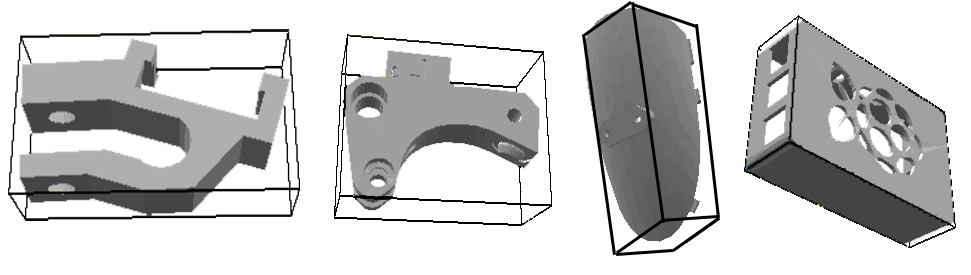
\includegraphics[height=50pt, trim=333 48 418 33, clip]{figures/Industrial Prismatic Cavity Task Objects.png}}%
  \hfill%
  \subcaptionbox*{Shield Part}[42pt]{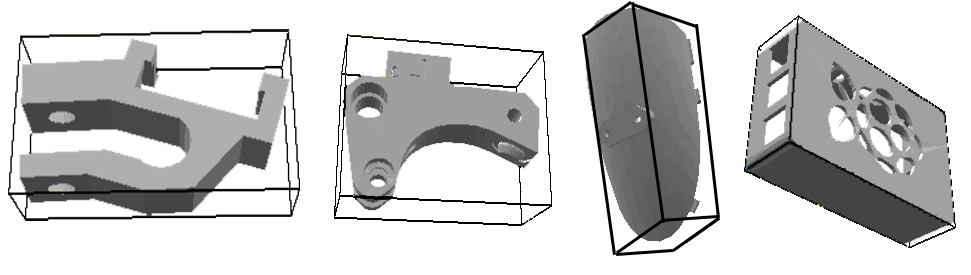
\includegraphics[height=50pt, trim=581 18 250 0, clip]{figures/Industrial Prismatic Cavity Task Objects.png}}%
  \hfill%
  \subcaptionbox*{Endstop Holder}{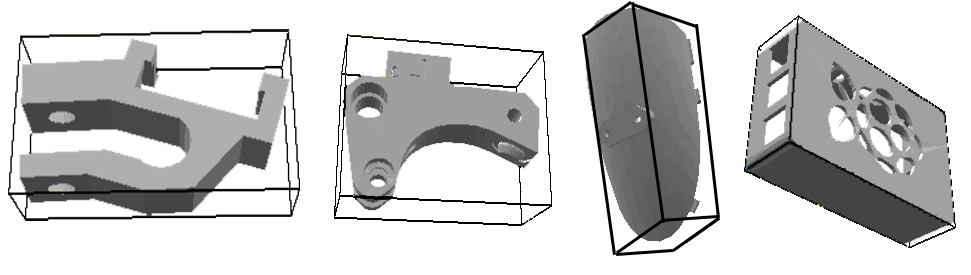
\includegraphics[height=50pt, trim=7 53 670 28, clip]{figures/Industrial Prismatic Cavity Task Objects.png}}%
  \hfill%
  \subcaptionbox*{Raspberry Pi Case}[62pt]{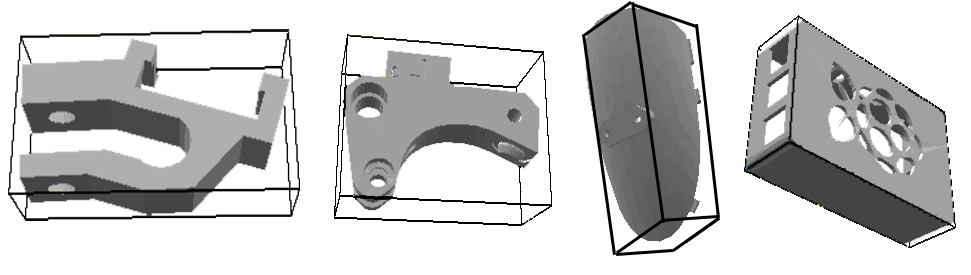
\includegraphics[height=50pt, trim=743 26 14 14, clip]{figures/Industrial Prismatic Cavity Task Objects.png}}
  \caption{\textbf{Examples of Novel Objects for Kit-Net Simulation Experiments: }
%   From left to right, these are the endstop holder, industrial part, shield part, and a raspberry pi case. 
  The four test objects are unseen during training and have eccentricity greater than 2, meaning their minimum volume bounding boxes are narrow and long. An outline of the corresponding minimum volume bounding box is shown around each part.}
  \label{fig:prism-task-eval-objects}
\end{figure}

\begin{figure}[t]
  \centering
  \vspace{8pt}
  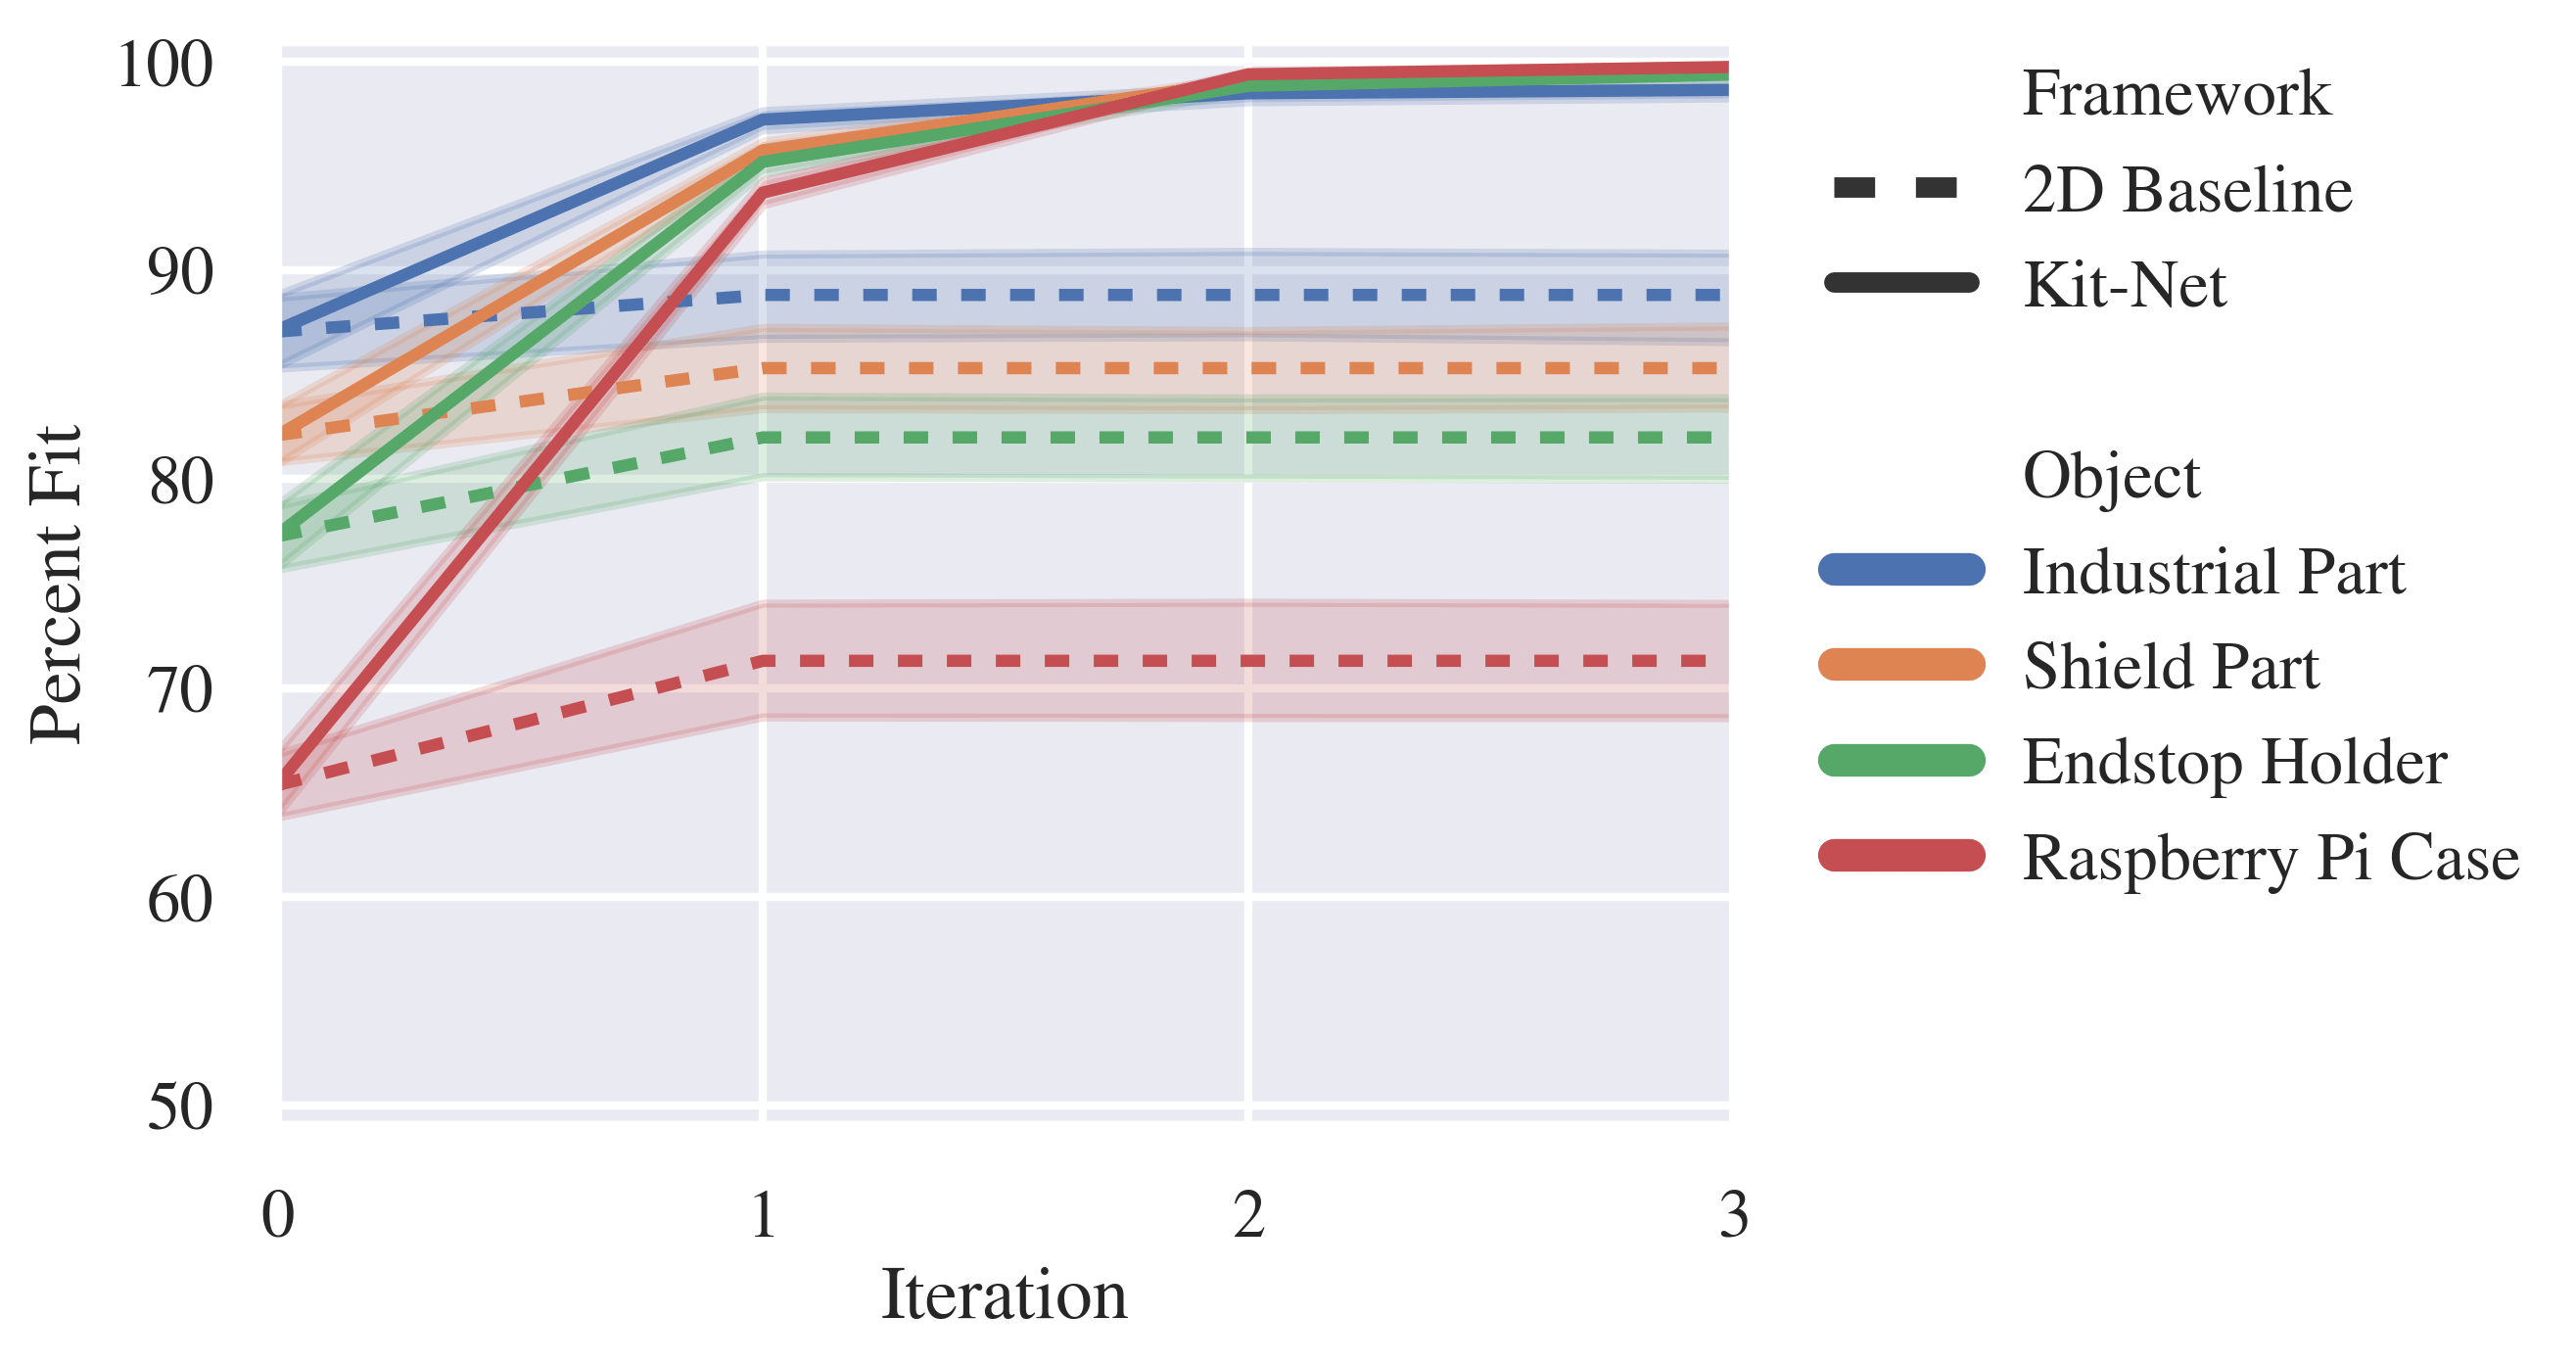
\includegraphics[width=0.48\textwidth]{figures/percent_fit_controller_runs_v6.png}
  \caption{\textbf{Kit-Net Simulation Results: } We visualize data from 100 runs on each of the 4 objects shown in Figure~\ref{fig:prism-task-eval-objects}. All objects require a 30\degree~rotation to be in alignment with the prismatic target at iteration 0, but their initial percent fits differ due to different eccentricities. Results suggest that Kit-Net is able to successfully align all 4 objects with their respective prismatic cavities while the baseline, which restricts itself to 2D rotations, performs significantly worse on all 4 objects.}
  \label{fig:percent-fit-runs}
\end{figure}



% \begin{figure}
%   \centering
%   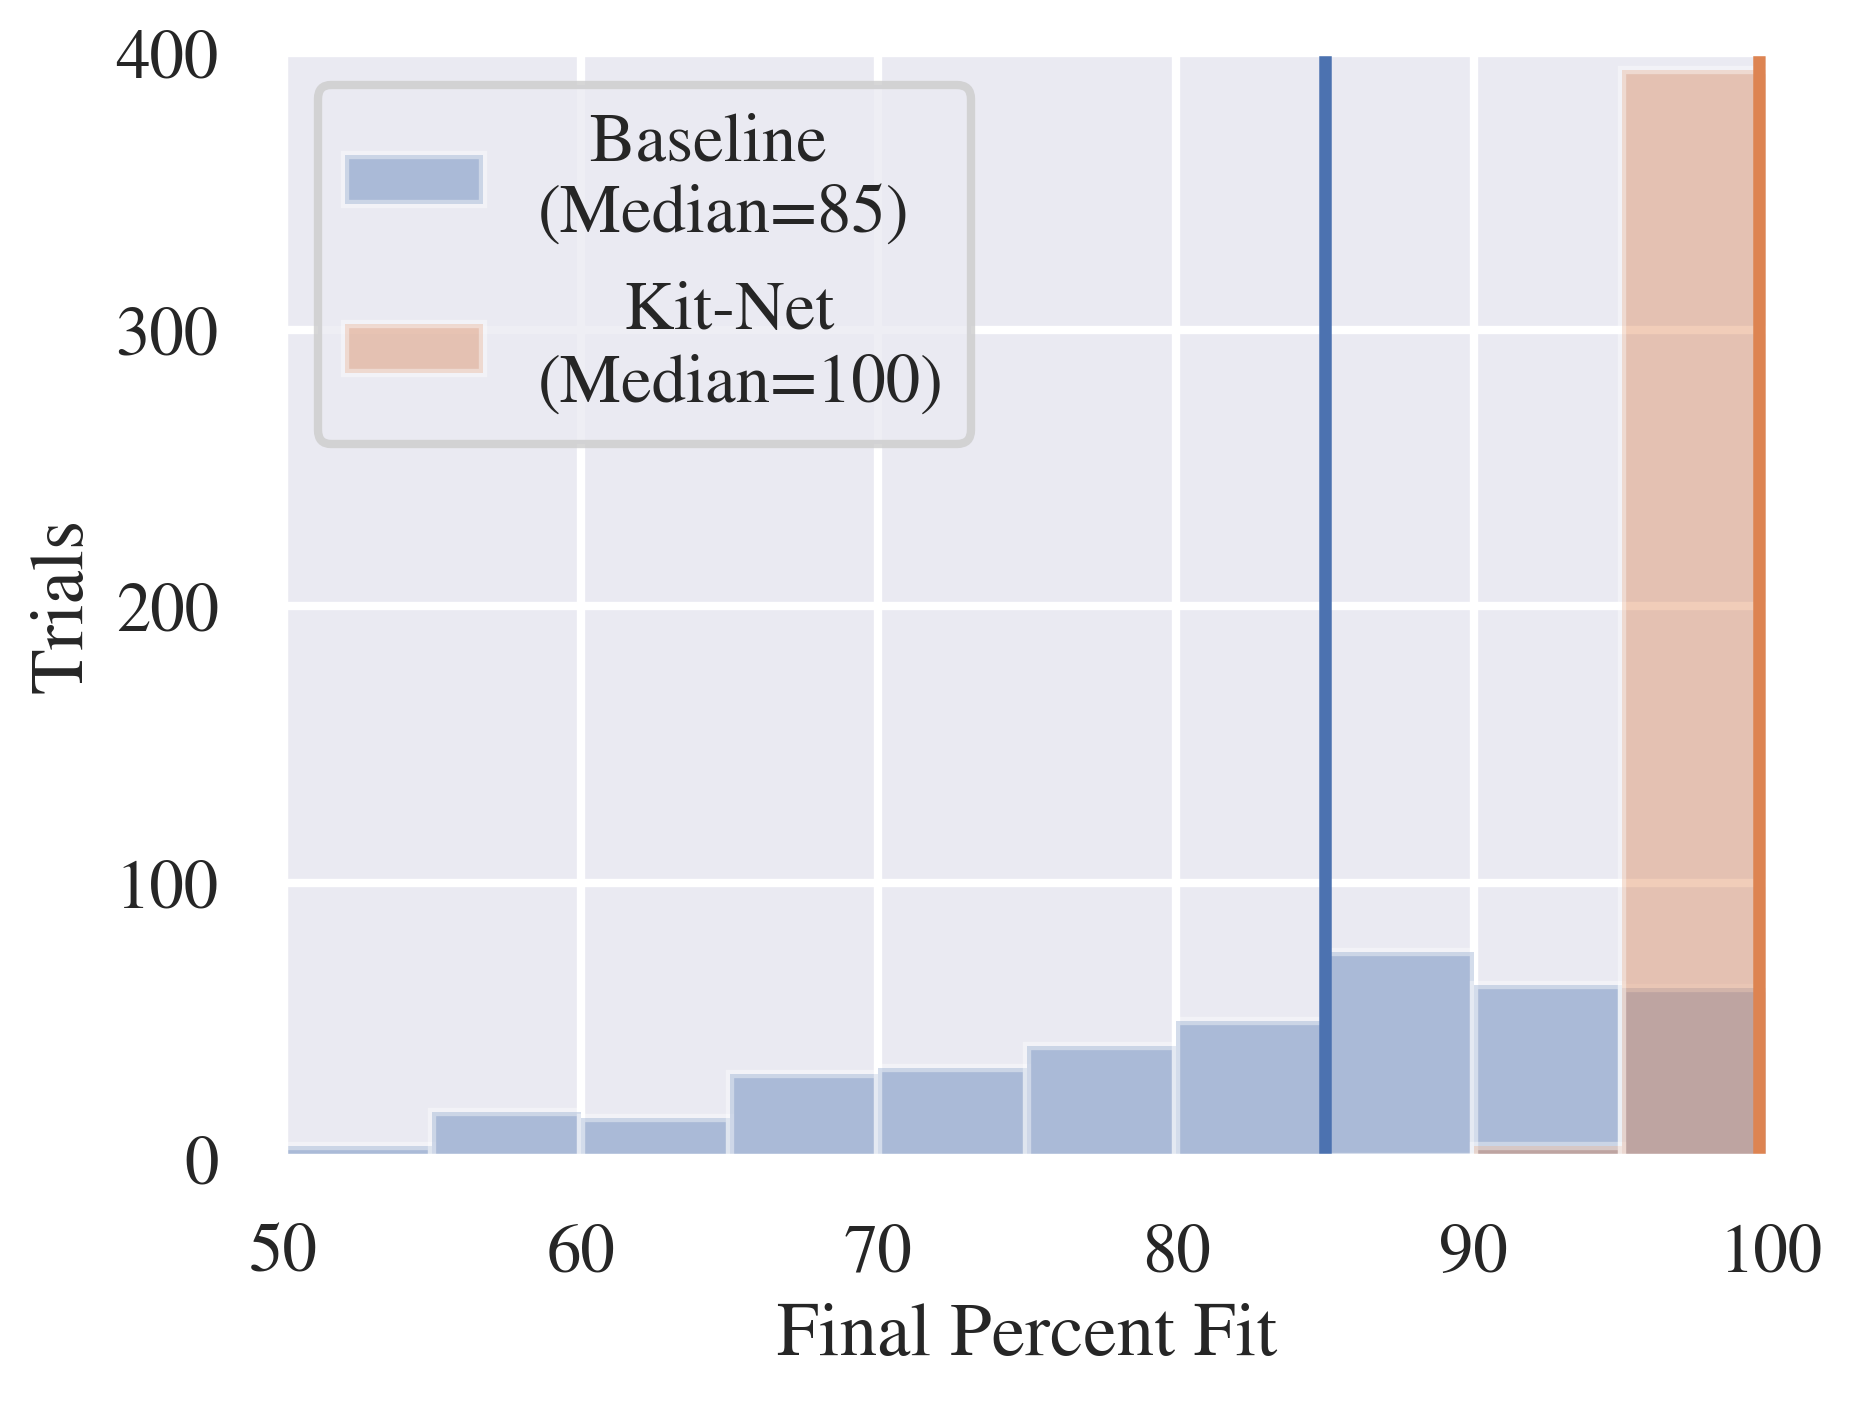
\includegraphics[width=0.9\linewidth]{figures/percent_fit_controller_hist_v3.png}
%   \caption{Kit-Net with the prismatic cavity targets. The controller takes incremental steps based on $\hat{{_s}R^g}$ and moves closer towards the target prism in up to 5 steps. We plot a histogram of the final percent fit and see that the median is 99.4\%, suggesting that Kit-Net can effectively orient novel objects towards a prismatic target for insertion. \AB{what information does this Figure provided that isn't already in Figure~\ref{fig:percent-fit-runs}?} \MD{agree, we can probably remove!}}
%   \label{fig:percent-fit-hist}
% \end{figure}

%\input{includes/5.2-positive-cavity}
%\input{includes/5.3-negative-cavity}

% \begin{figure}
%   \centering
%   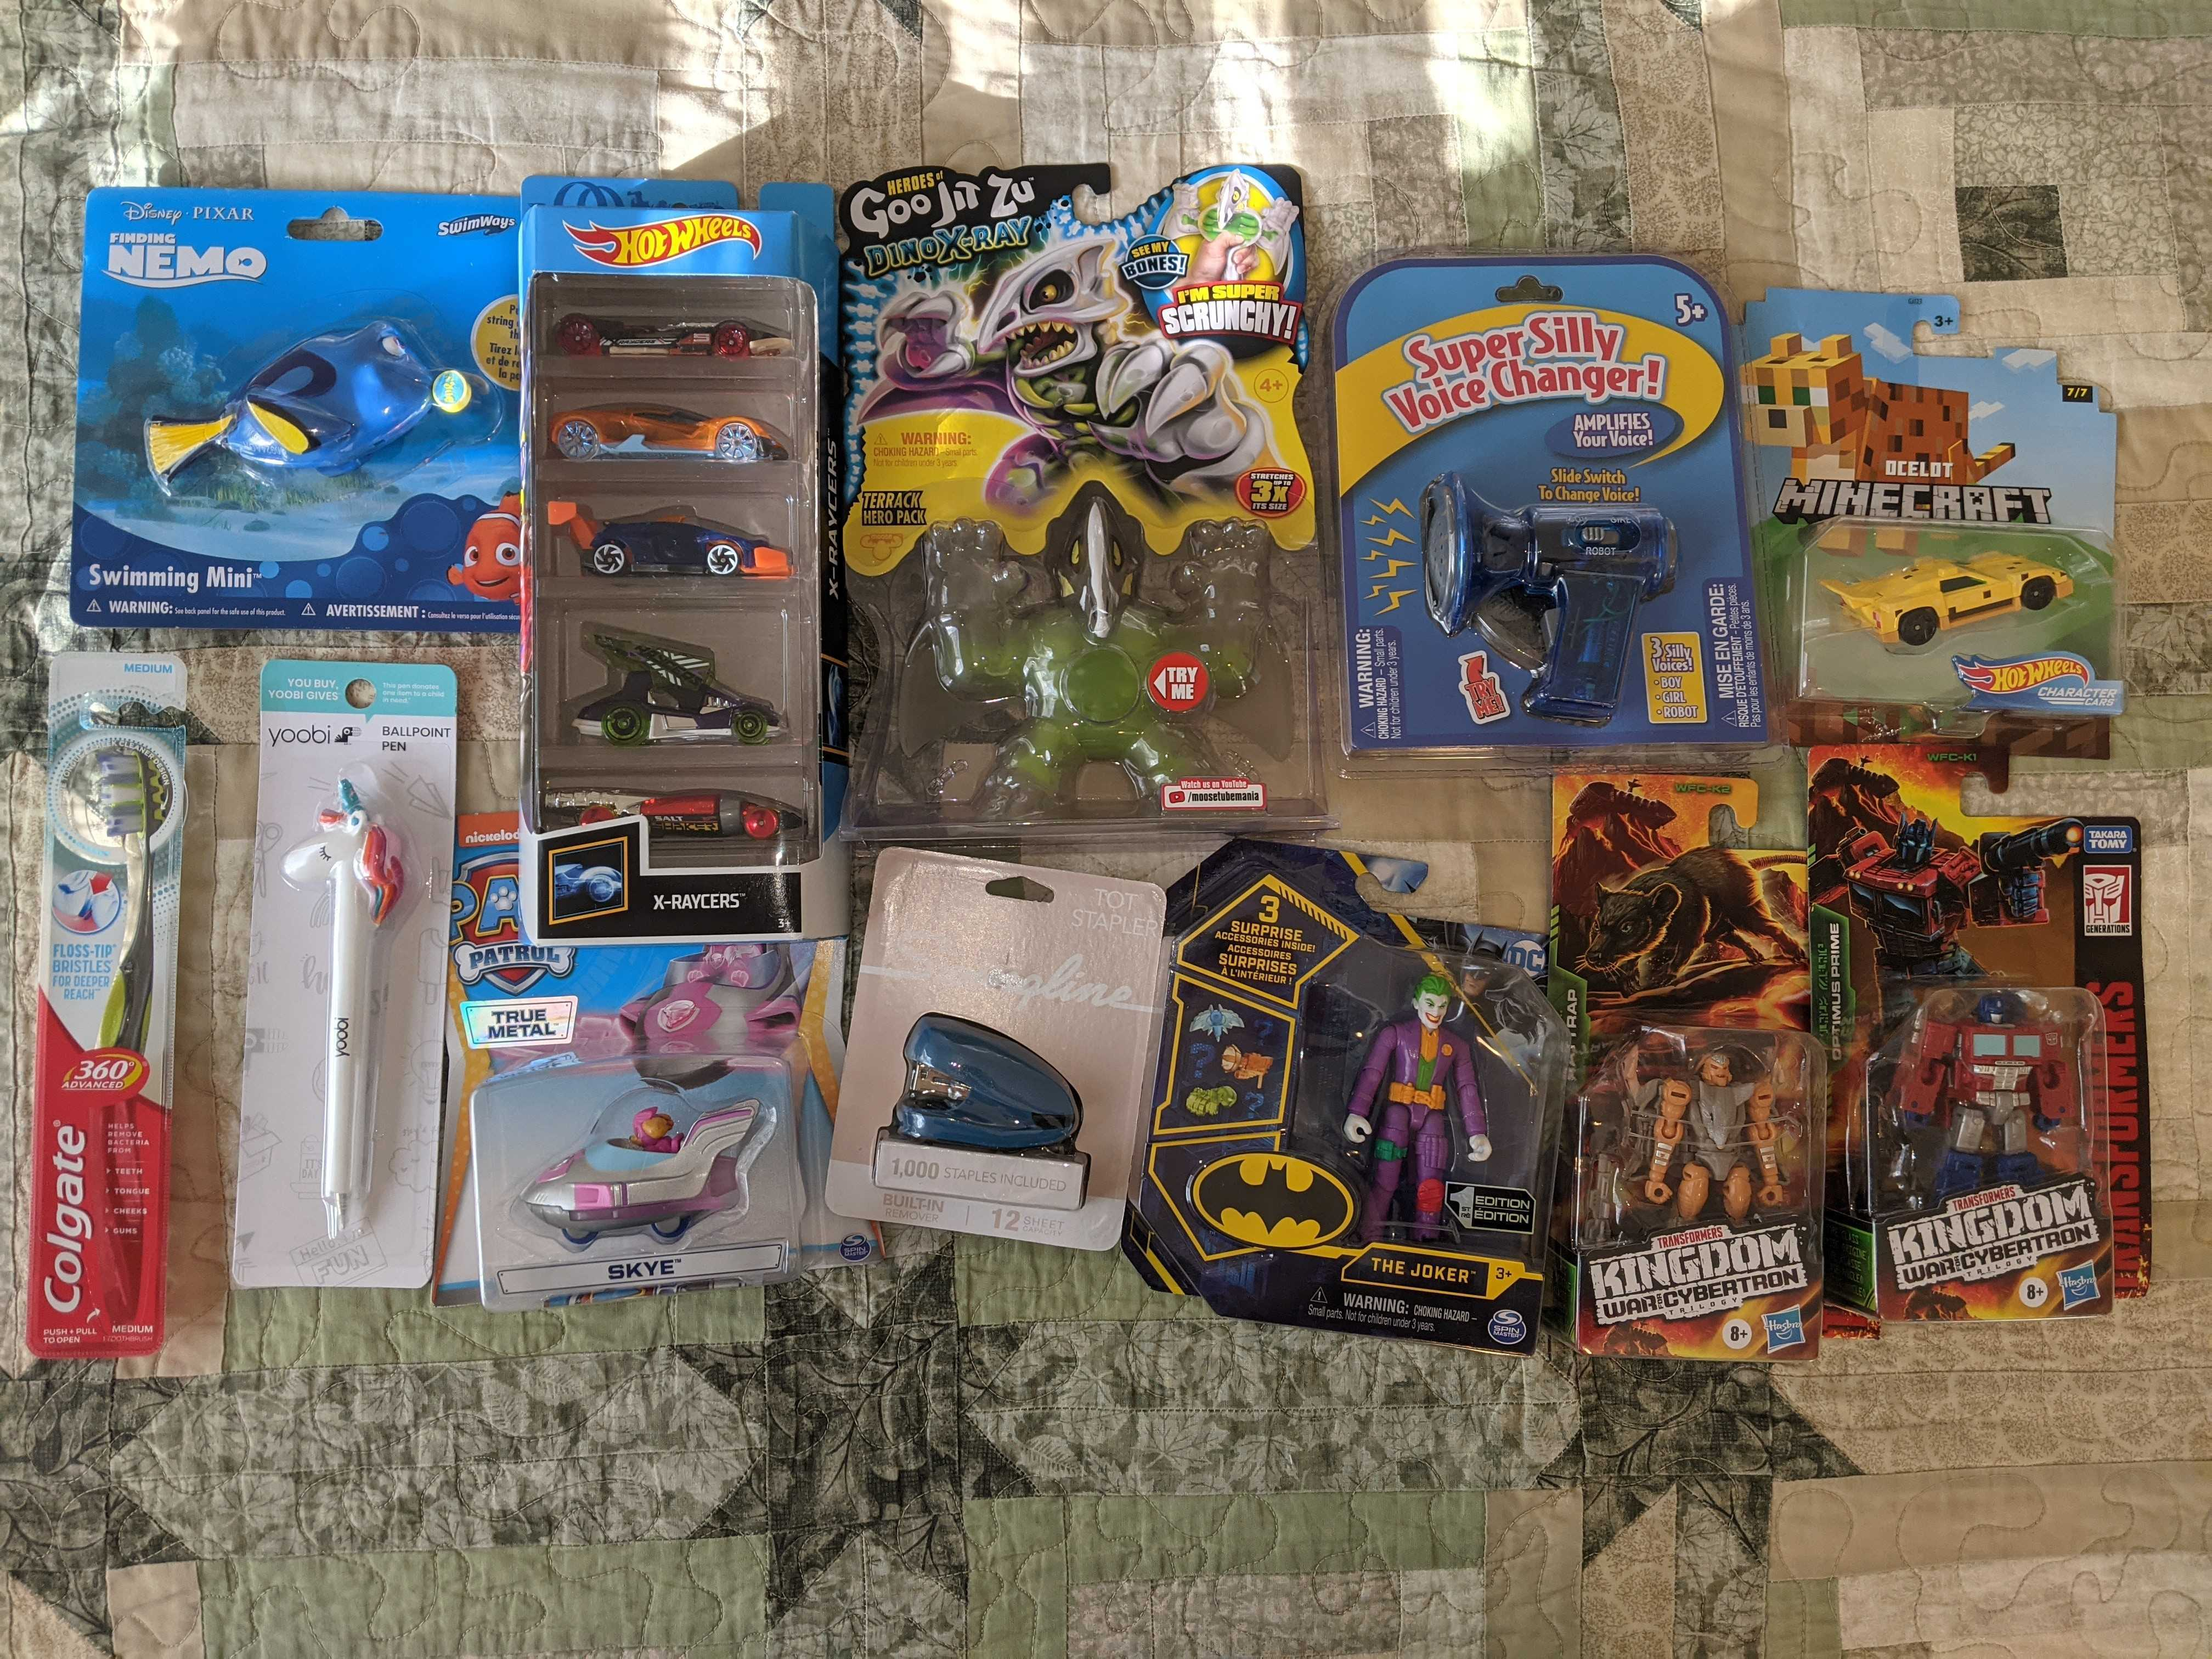
\includegraphics[width=0.48\textwidth]{figures/toy-clamshells.jpg}
%   \caption{Packaged toys used for kitting cavity insertion task. We bought these at Target, and observe that these objects require accurate orientation in order to insert the object into the cavity. \todo{Proper lighting, top down, maybe have kitting next to object.}}
%   \label{fig:toy-clamshells}
% \end{figure}

% \subsection{Clay Embedding}
% \label{subsec:clay}
% We can create our own impression of an object onto modelling clay, and use this impression as a target for insertion. We can take a depth image of the cavity and negate it in order to get a positive depth image of an object target. We then orient and insert the object in a similar way as \ref{subsec:real-positive}.



\section{Physical Experiments}
\label{sec:physical-experiments}
Our previous experiments studied the effectiveness of Kit-Net for insertion tasks involving prismatic cavities. However, as shown in Fig.~\ref{fig:clamshell-objects} and Fig.~\ref{fig:clamshell-cavities}, many physical kitting tasks involve non-prismatic cavities. In this section, we study how Kit-Net can be used to kit objects in physical trials using depth images of the types of cavities shown in Fig.~\ref{fig:clamshell-cavities}. We call these \emph{conformal cavities}, as they ``conform" to some degree to the object shape. 

In these experiments we use a quaternion prediction network trained to predict the quaternion that will rotate a simulated depth image of an object to another simulated depth image of the same object in a different pose. We propose two possible methods for applying this trained network to kitting. Our first method is designed to work well with the clamshell cavities shown in Fig.~\ref{fig:clamshell-cavities}. Rather than image the hole of the cavity, we define a \emph{convex conformal cavity} to be the depth image of the inverted cavity. To obtain these depth images, we flip the cavity so the hole is pointing down and take a depth image of the positive mass of the cavity. The left image in Fig.~\ref{fig:clamshell-cavities} shows examples of these convex conformal cavities. Our second method works with a \emph{concave conformal cavity}, like that shown in Fig.~\ref{fig:mug-cavity-2} and the right image in Fig.~\ref{fig:clamshell-cavities}, that are formed as impressions into a surface. These types of cavities cannot simply be flipped upside down to obtain a depth image of their shape. Instead, we take a depth image of the actual cavity (where the cavity has negative mass) and rotate it 180\degree~about its principal axis.

We discuss the results for applying Kit-Net to novel convex conformal cavities in Section~\ref{subsubsec:real-positive} and to novel concave conformal cavities Section~\ref{subsubsec:real-negative}.
For the physical kitting experiments we measure success using a binary success metric for insertion by visually inspecting whether or not the object is completely contained in the target cavity.

\subsection{Physical Kitting into Convex Conformal Cavities}
\label{subsubsec:real-positive}

\begin{figure}[t]
  \vspace{8pt}
  \centering
  \begin{tikzpicture}[label/.style={inner sep=4pt, rounded corners=2pt, color=white, fill=black, fill opacity=0.25, text opacity=1, align=center, font=\footnotesize, yshift=2pt}]
    \node [inner sep=0] (img) {%
     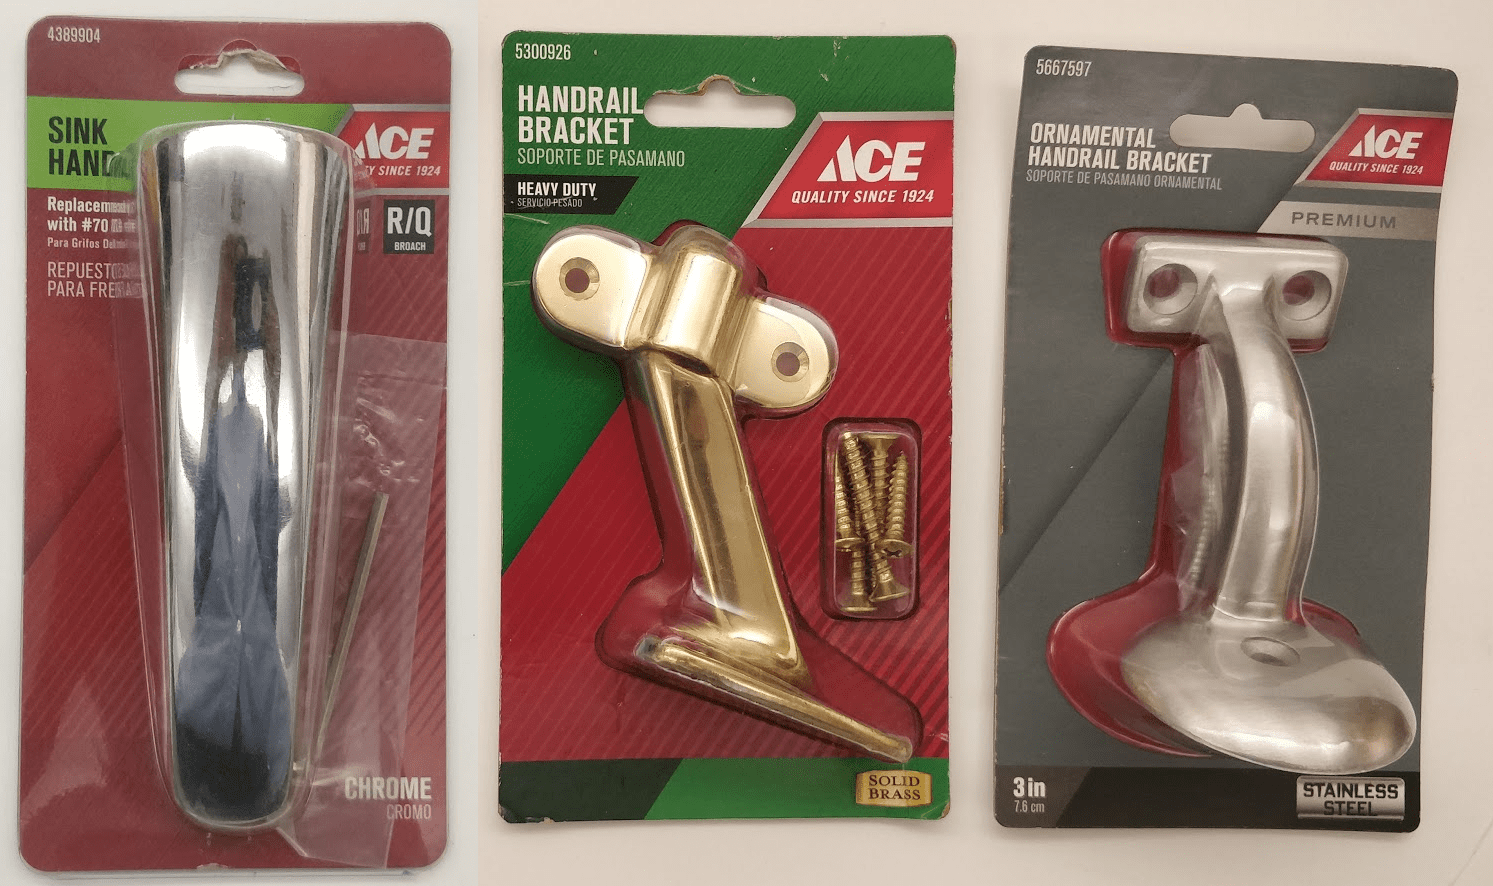
\includegraphics[width=\columnwidth]{figures/Three_Industrial_Objects.png}};
    \node [label, anchor=south west, xshift=14pt] at (img.south west) { Sink handle };
    \node [label, anchor=south, xshift=-4pt] at (img.south) { Handrail bracket };
    \node [label, anchor=south east, xshift=-14pt] at (img.south east) { Ornamental \\ handrail bracket };
  \end{tikzpicture}
  \caption{\textbf{Objects for Kit-Net Physical Experiments: }We use 3 packaged industrial objects that can be commonly found in a hardware store. 
   These objects were selected for their complex geometries, making precise orientation critical for effective kitting.}
  \label{fig:clamshell-objects}
\end{figure}

\begin{figure}[t]
  \centering
  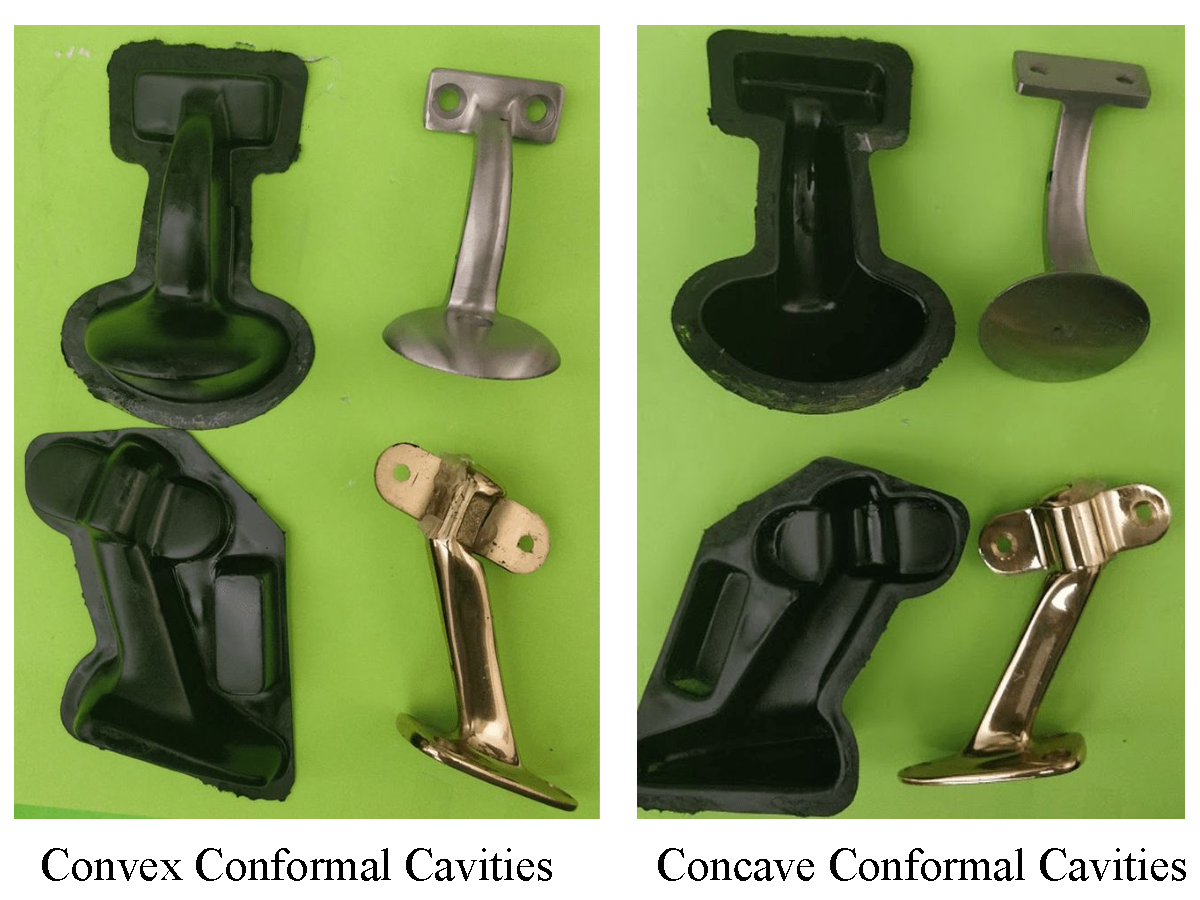
\includegraphics[width=\columnwidth]{figures/convex_concave_examples.pdf}
  \caption{\textbf{Examples of Physical Kitting Cavities: }The handrail bracket (bottom) and the ornamental handrail bracket (top), next to the corresponding convex cavity (left) and concave cavity (right).}
  \label{fig:clamshell-cavities}
\end{figure}

We also evaluate Kit-Net in physical kitting trials on an ABB-YuMi robot with a Photoneo depth camera, shown in Fig.~\ref{fig:splash}, using 4 packaged objects widely available in hardware stores and which are unseen during training (Fig.~\ref{fig:clamshell-objects}). %Figure~\ref{fig:toy-clamshells} visualizes packed toys widely available in retail stores. 
To prepare objects for kitting, we carefully extract each tool and kitting shell from its packaging and spray paint the shell to facilitate depth sensing as shown in Fig.~\ref{fig:clamshell-cavities}. We then place the kitting cavity open end down and image the cavity to generate $I^g$ before flipping it to expose its opening for the insertion task. For each trial, we insert the object into the cavity by hand, grasp it using the robot's suction gripper, translate it to be directly under the camera, and apply a random rotation of either $30\degree$ or $60\degree$, uniformly sampled from $SO(3)$ to simulate grasping the object from a bin in a non-uniform pose. Then, we flip the object such that the object faces the overhead depth camera and the suction cup grasp is occluded from the camera by the object. This process is illustrated in Fig.~\ref{fig:splash}. 

Kit-Net then orients the object using the learned controller, and matches centroids between the object and cavity for insertion before flipping it again and attempting to kit it. Table~\ref{table:positive-results} shows the number of successful kitting trials (out of 10 per object) of Kit-Net and the 2D baseline across 3 objects. We report a kitting trial as successful if the object is fully contained within the cavity from visual inspection. We observe that Kit-Net outperforms the baseline for 30\degree~initial rotations on 2 of the 3 objects, performing similarly to the baseline on the sink handle. We find that Kit-Net significantly outperforms the baseline on all objects for 60\degree~initial rotations.

Kit-Net's main failure modes are due to errors in the centroid matching procedure, as illustrated in Fig.~\ref{fig:failure-modes}. On the 30 degree sink handle task, Kit-Net aligned it correctly every time, but the centroid matching had it about ~0.5\,cm off, and there is no slack at the top of the cavity.


%\SJ{We can also add a table with success rate for each physical object that we tested on. Also comparison table with other methods using similar techniques example with- Zakka's method. In that case we can use similar items and also do a fit percentage comparison} 
% However, while \citet{zeng2020transporter} framed a 2D pick-and-place task given an image of an object and its place target by computing ${_s}T^g \in SE(2)$ through an efficient cross-convolution operation on GPU, we consider the best ${_s}T^g \in SE(2)$ by computing the best ${_s}R^g \in SO(2)$ that minimizes the chamfer distance between the point cloud representations of $I^s$ and $I^g$. 

\begin{table}[h]
\centering
\begin{tabular}{l c c c}\toprule 
 Object & Angle & 2D Baseline & Kit-Net \\
 \midrule
 Handrail bracket & 30\degree & 3/10 & \bf 10/10 \\ 
 Ornamental handrail bracket & 30\degree & 8/10 &  \bf 10/10 \\
 Sink handle & 30\degree & \bf 4/10 & 3/10 \\
 \addlinespace
 Handrail bracket & 60\degree & 1/10 & \bf 9/10 \\ 
 Ornamental handrail bracket & 60\degree & 2/10 & \bf 7/10 \\
 Sink handle & 60\degree & 0/10 & \bf 7/10 \\
 \bottomrule
\end{tabular}
\caption{\textbf{Physical Experiments Results for Convex Cavities: }We report the number of successful kitting trials for Kit-Net and the 2D baseline over 10 trials for 3 previously unseen objects with initial rotations of 30\degree and 60\degree. Results suggest that Kit-Net significantly outperforms the 2D baseline for initial rotations of 60\degree and outperforms the baseline for two out of three objects for initial rotations of 30\degree.}
\label{table:positive-results}
\end{table}
\subsection{Physical Kitting into Concave Conformal Cavities}
\label{subsubsec:real-negative}
%The positive cavity task provides a detailed depth image, but requires the cavity to first be presented at a flipped, 180\degree~rotation for imaging, which may not be feasible in an industrial environment. [this is a minor detail: omit. -KG 3/18]
Here, we perform the same experiment as in Section~\ref{subsubsec:real-positive}, but instead generate $I^g$ directly from an image of the cavity without flipping. Precisely, we segment out the cavity from an overhead depth image, deproject the depth image into its point cloud representation, and rotate the point cloud 180\degree~around its center of mass. Then, we project the rotated point cloud to the depth image $I^g$. %This process is illustrated in Fig.~\ref{fig:rotated-cavity}.

\begin{table}[h]
\centering
 \begin{tabular}{l c c c}\toprule
 Object & Angle & 2D Baseline & Kit-Net \\
 \midrule
 Handrail bracket & 30\degree & 0/10 & \bf 9/10 \\ 
 Ornamental handrail bracket & 30\degree & 0/10 & \bf 7/10 \\
 Sink handle & 30\degree & 1/10 & \bf 3/10 \\
 \addlinespace
 Handrail bracket & 60\degree & 0/10 & \bf 7/10 \\ 
 Ornamental handrail bracket & 60\degree & 0/10 & 0/10 \\
 Sink handle & 60\degree & 1/10 & \bf 4/10 \\
 \bottomrule
\end{tabular}
\caption{\textbf{Physical Experiments Results for Concave Cavities: }We report the number of successful kitting trials for Kit-Net and the 2D baseline over 10 trials for 3 previously unseen objects with initial rotations of 30\degree and 60\degree. Results suggest that Kit-Net significantly outperforms the baseline in all settings except for the handrail bracket with an initial rotation of 60\degree, for which neither Kit-Net nor the baseline can successfully kit the object.}
\label{table:negative-results}
\end{table}

Table~\ref{table:negative-results} shows results from experiments with 3 novel objects from Fig.~\ref{fig:clamshell-objects} across 10 controller rollouts. We observe that Kit-Net outperforms the baseline for initial rotations of both 30 and 60 degrees on the handrail bracket and sink handle, and for an initial rotation of 30 \degree for the ornamental handrail bracket. For the ornamental handrail bracket, the depth image from the concave cavity is low quality as shown in Fig.~\ref{fig:failure-modes} (center image), causing Kit-Net to fail when the object is 60 degrees away the correct insertion orientation. We examined this failure and found that it occurs because the cavity for the neck of the bracket is very thin, making it difficult to obtain a good depth image. Kit-Net also has low performance on the sink handle due to small errors in centroid matching, as discussed in the prior section. Fig.~\ref{fig:failure-modes} (bottom left) shows an example failure case where the sink handle is correctly oriented but the translation is slightly off. There were also occasional cases (Fig.~\ref{fig:failure-modes} (top left)) where the suction gripper occludes the handle of the ornamental handrail bracket. In these cases, the robot can only see the base, resulting in failure.

% \begin{figure}
  \centering
  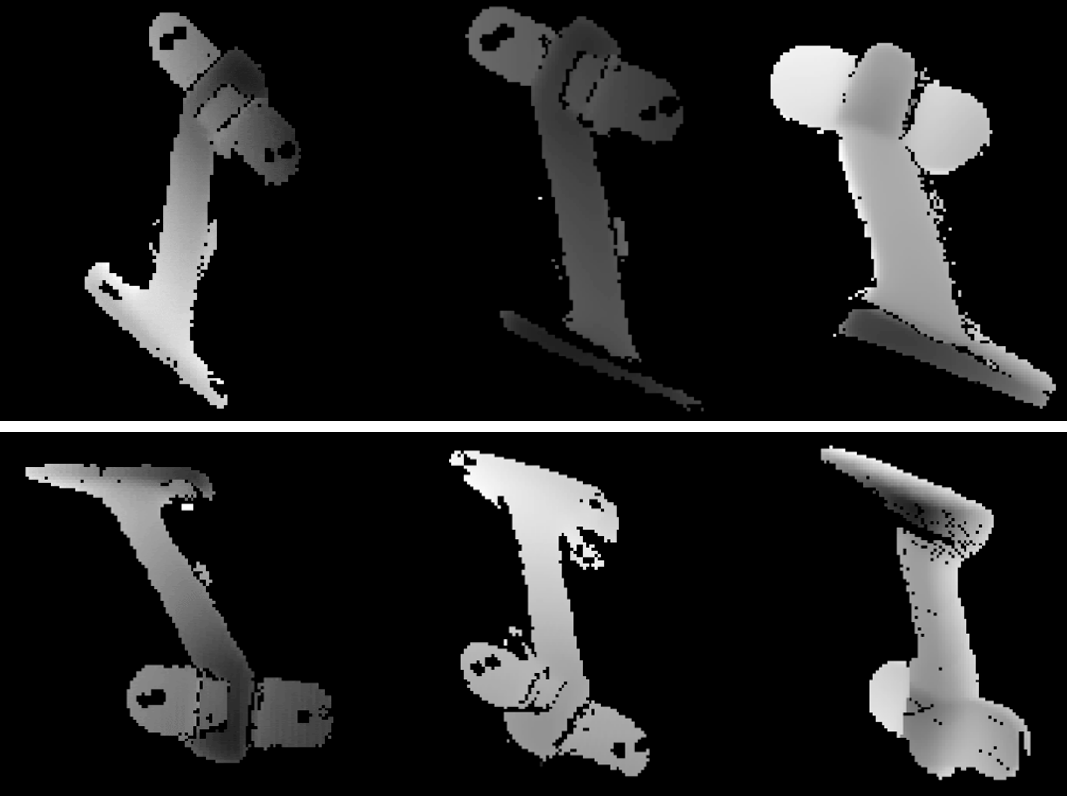
\includegraphics[width=0.48\textwidth]{figures/Orientation.PNG}
  \caption{\AB{this figure needs some labels, eg. $I^s$, $\hat{I}^g$, $I^g$}\textbf{Reorienting Objects with Kit-Net: }Kit-Net aligns objects from $I^s$ (left) to $\hat{I}^g$ (middle) given both positive (top right) and negative (bottom right) goal images $I^g$ by estimating ${_s}\hat{t}^g \in SE(3)$. Positive goal images are generated as described in Section~\ref{subsubsec:real-positive} while negative goal images are generated as described in Section~\ref{subsubsec:real-negative}.}
  \label{fig:Kit-Net-to-cavity}
\end{figure} OMIT -KG 3/18

\begin{figure}[t]
  \vspace{8pt}
  \centering
  % "Break between images" -KG
%   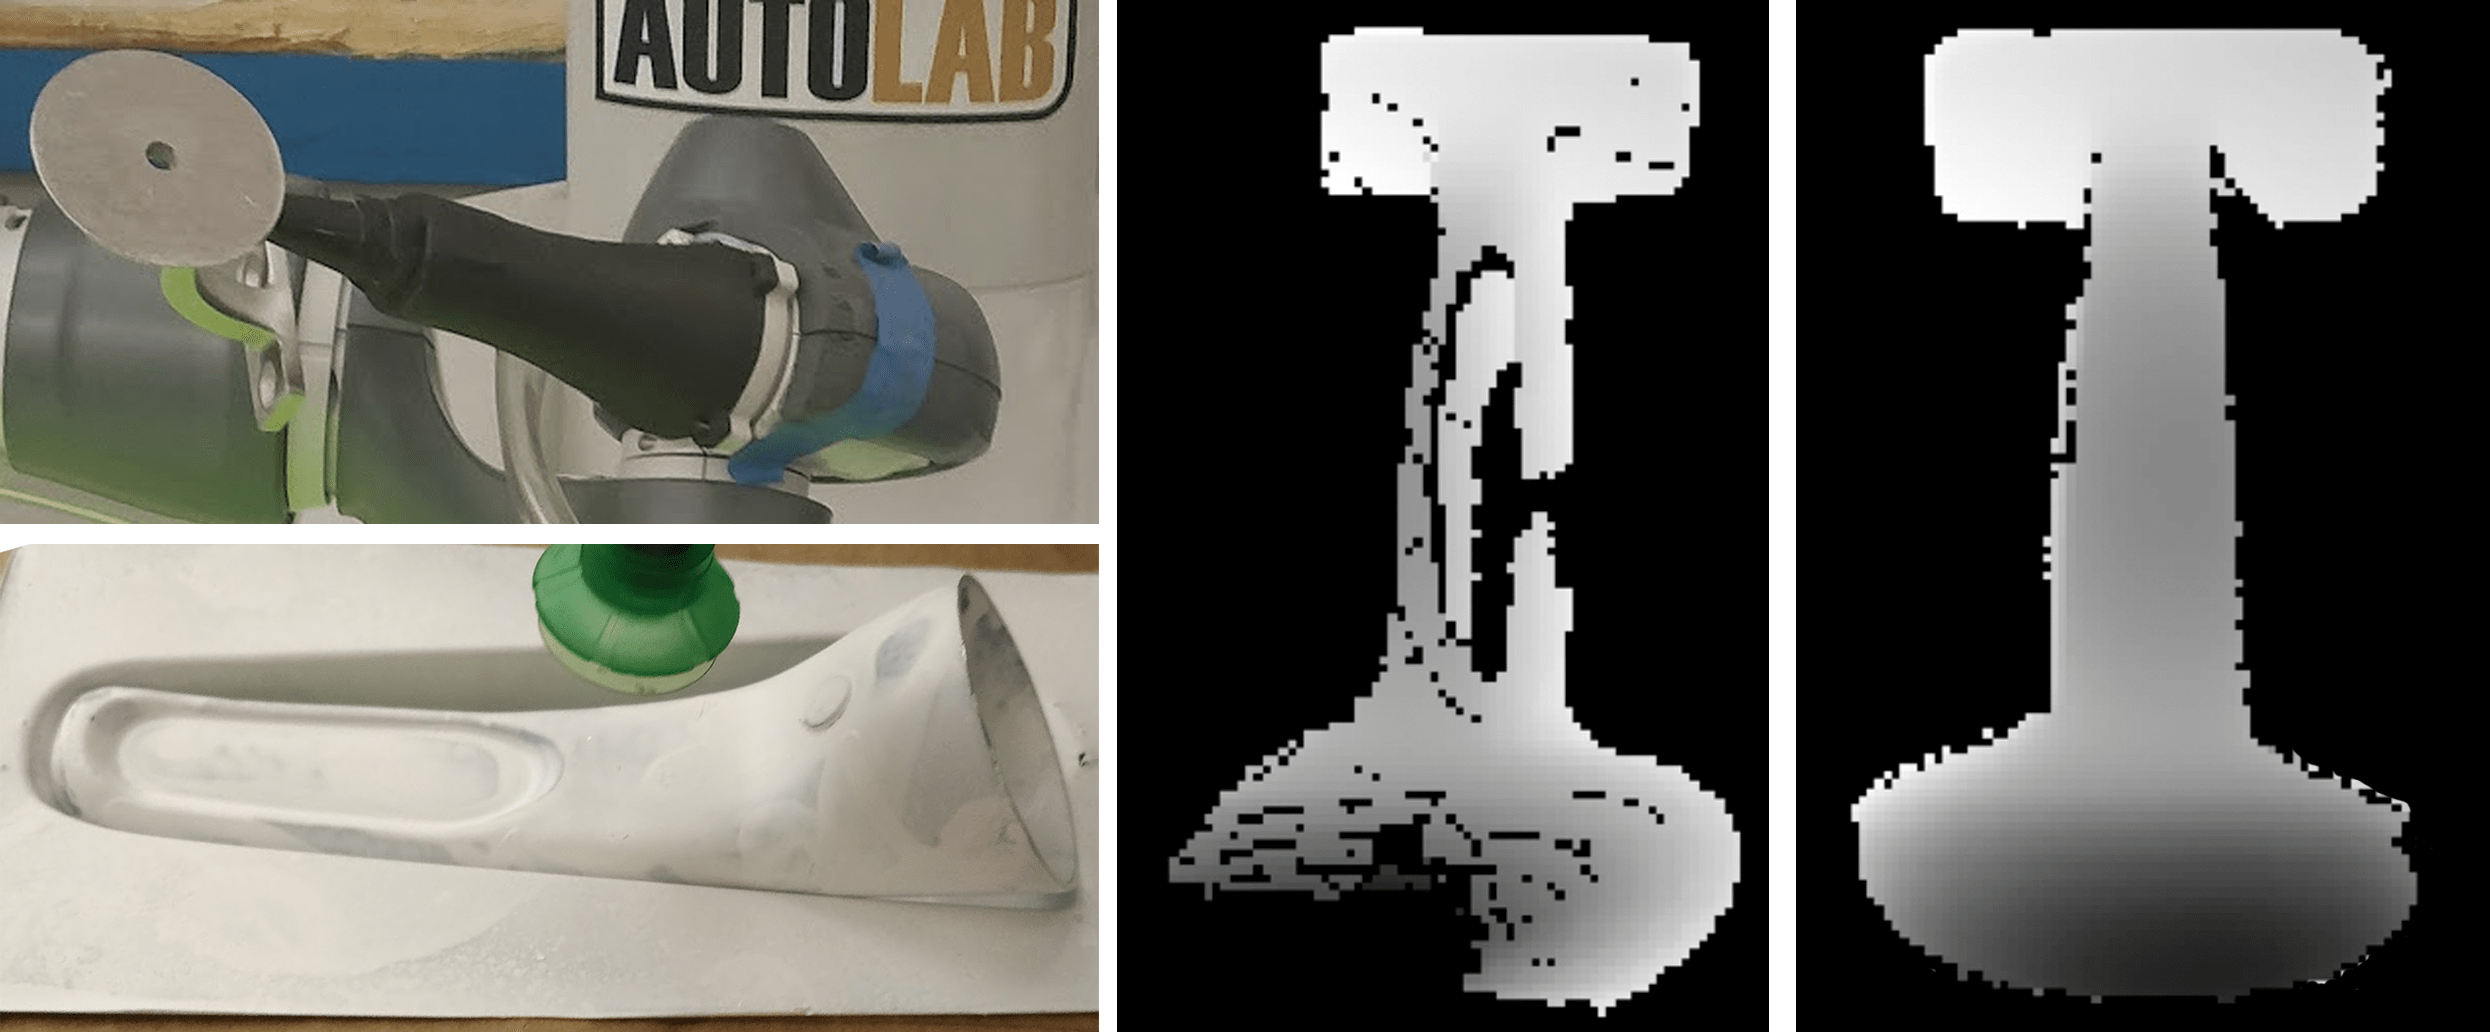
\includegraphics[width=0.48\textwidth, trim=0 488 0 0, clip]{figures/Failure Cases.png} \\[2pt]
%   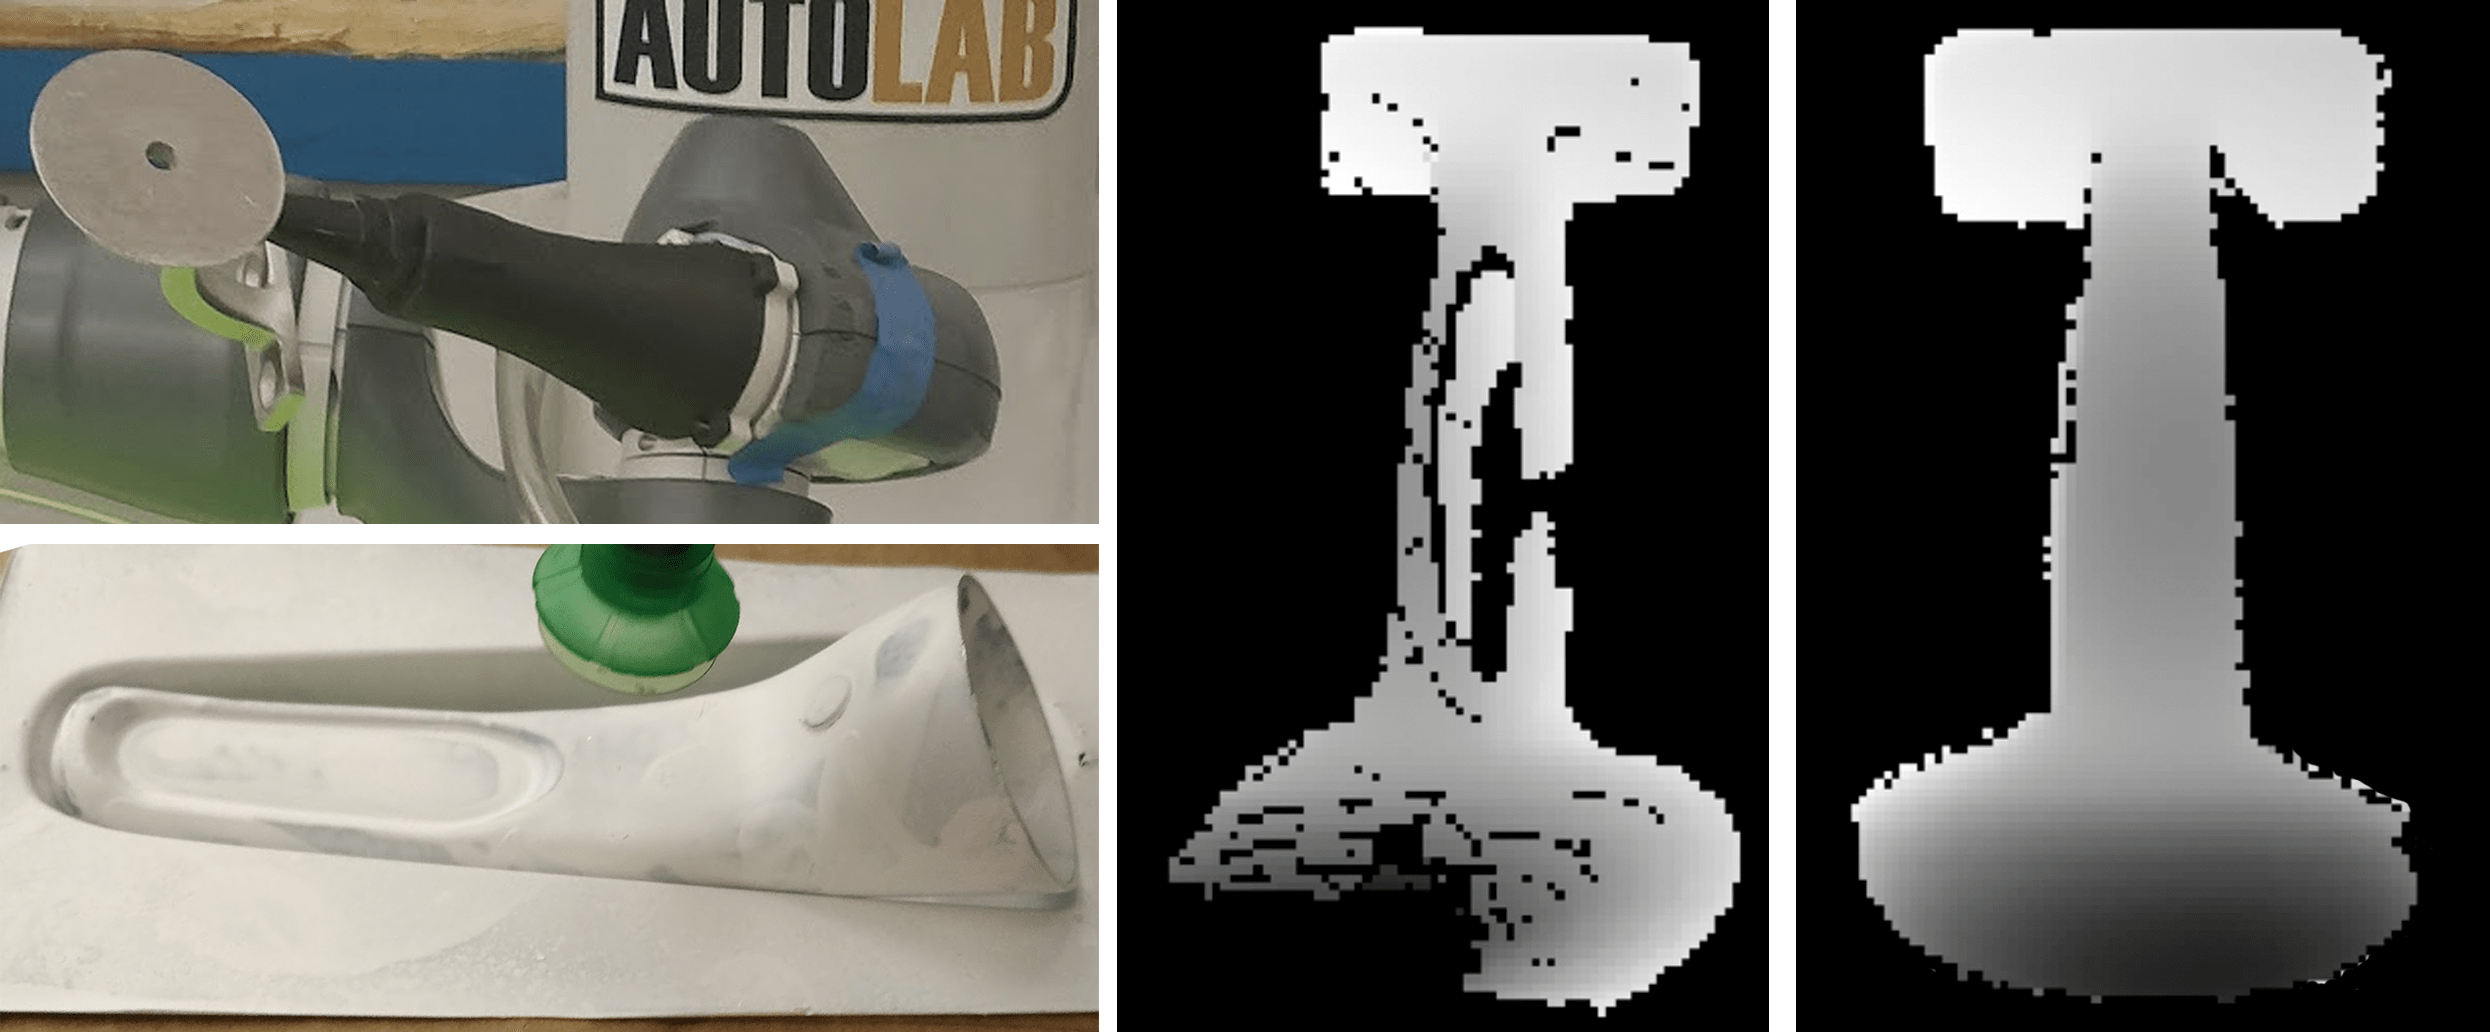
\includegraphics[width=0.48\textwidth, trim=0 0 0 636, clip]{figures/Failure Cases.png}
  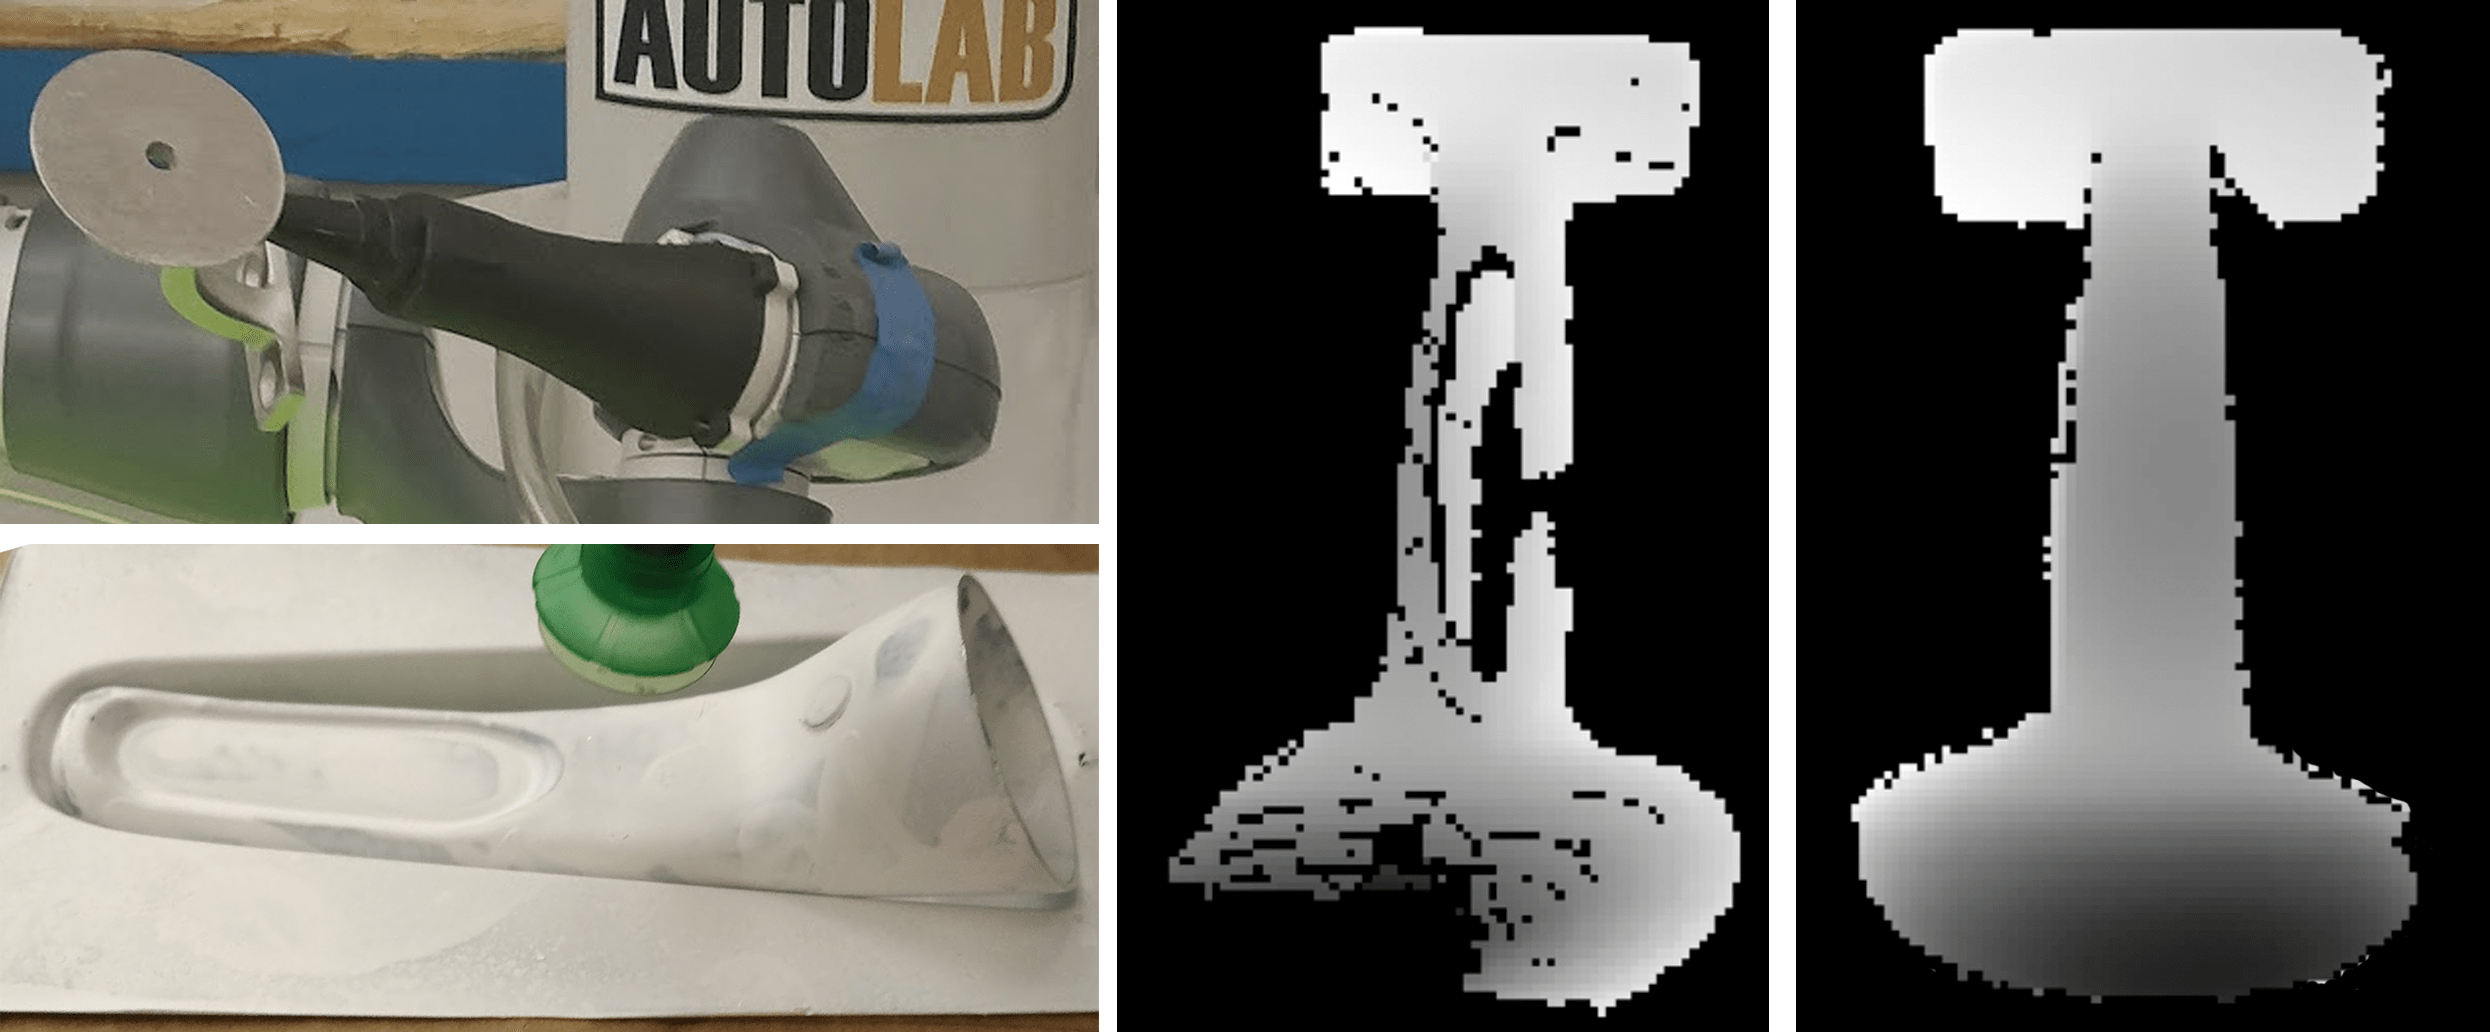
\includegraphics[width=0.48\textwidth]{figures/Failure Cases.png}
  \caption{\textbf{Kit-Net Failure Cases: } The top-left image shows a configuration of the ornamental handrail bracket
  %that results in self-occlusion; the downward-facing depth camera cannot image
  where the suction gripper occludes
  the handle below the base. The bottom-left image shows the sink handle. Although Kit-Net was able to orient the handle correctly for insertion, the centroid matching had a small error in estimating translation and the cavity does not have enough slack to be properly inserted. The center and right images show depth images for the ornamental handrail bracket for the concave conformal cavity and convex conformal cavity, respectively.
  %using the process described in \ref{subsec:real-negative}, and the right image shows the depth image of the cavity positive as described in \ref{subsec:real-positive}.
  The inside of the concave cavity is very thin and the angle of the camera makes it hard to perfectly image it, resulting in a poor depth image (center image). % using the method of \ref{subsec:real-negative}.
  This leads to 0 successes for both the baseline and for Kit-Net when the initial rotation is 60\degree{} away from the desired rotation for kitting.}
  \label{fig:failure-modes}
\end{figure}


% \begin{figure}
  \centering
  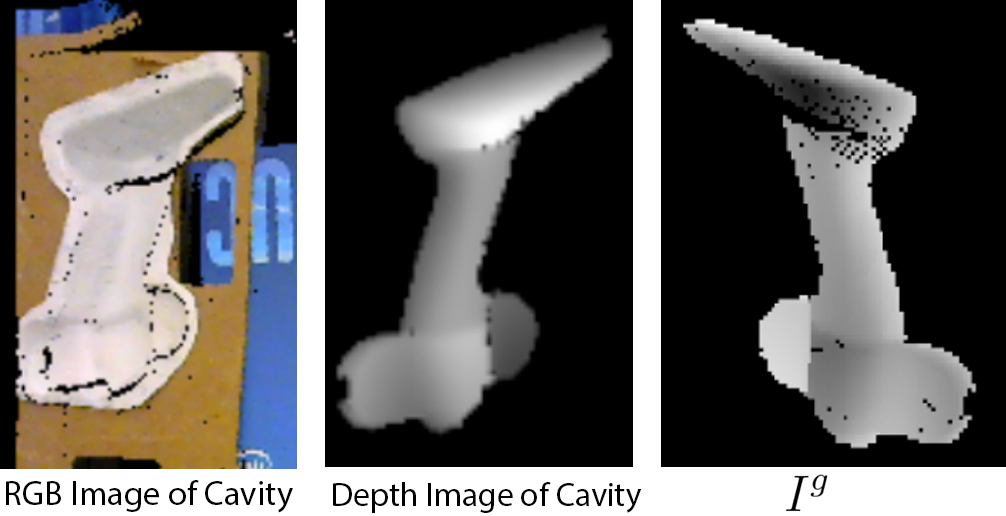
\includegraphics[width=0.48\textwidth]{figures/Rotated_Negative.png}
  \caption{\textbf{Generating Negative Goal Images: }After taking the original image (left), we segment out all parts that don't belong to the cavity (middle). Then, we project from depth to point cloud, rotate the pointcloud about its centroid, and deproject to depth image to get $I^g$ (right).}
  \label{fig:rotated-cavity}
\end{figure}
 OMIT -KG 3/18

\section{Discussion and Future Work}
\label{sec:discussion}
We present Kit-Net, a framework that uses self-supervised deep learning in simulation to kit novel 3D objects into novel 3D cavities. Results in simulation experiments suggest that Kit-Net can kit unseen objects with unknown geometries into a prismatic target in less than 5 controller steps with a median percent fit of 99\,\%.
%Results in physical experiments suggest that Kit-Net can kit three novel 3D objects into novel 3D cavities 63\,\% of the time, outperforming a baseline that is limited to $SE(2)$ transformations and  succeeds only 18\,\% of the time. [LRBT!!! give Form2Fit first, THEN Kit-Net -KG 3/18]
In physical experiments kitting novel 3D objects into novel 3D cavities, Kit-Net is able to successfully kit novel objects 63\,\% of the time while a 2D baseline which only considers $SE(2)$ transforms only succeeds 18\,\% of the time.
%\textbf{Limitations and Future Work: }
%In this paper we do not consider suction grasps that would require the object to be regrasped (grasps that prevent both rotational alignment and insertion); however, this functionality may be necessary when grasping objects from a heap when $R^g$ exceeds 60\degree.
In future work, we will work to improve performance by using the predicted error from Kit-Net
%after an iteration time-out to detect the need for a regrasp. The object could then
to regrasp the object in a new stable pose~\cite{tournassoud1987regrasping,dafle2014extrinsic,danielczuk2020exploratory} before reattempting the kitting task, study Kit-Net's performance with other depth sensors, and apply Kit-Net to kit objects that are initially grasped from a heap \cite{murali20206,danielczuk2020x}.
% In future work, we will explore techniques to reduce the rotation prediction error for rotations with larger angles.
% only need acks in cam ready
\section{Acknowledgments}
\begin{scriptsize}
\noindent This research was performed at the AUTOLAB at UC Berkeley in affiliation with the Berkeley AI Research (BAIR) Lab, Berkeley Deep Drive (BDD), the Real-Time Intelligent Secure Execution (RISE) Lab, and the CITRIS ``People and Robots" (CPAR) Initiative. Authors were also supported by the Scalable Collaborative Human-Robot Learning (SCHooL) Project, a NSF National Robotics Initiative Award 1734633, and in part by donations from Siemens, Google, Toyota Research Institute, Autodesk, Honda, Intel, Hewlett-Packard and by equipment grants from PhotoNeo and Nvidia. This material is based upon work supported by the National Science Foundation Graduate Research Fellowship Program under Grant No. DGE 1752814. Any opinions, findings, and conclusions or recommendations expressed in this material are those of the authors and do not necessarily reflect the views of the sponsors.
% We thank our colleagues who provided feedback and suggestions, in particular .
\end{scriptsize}


% \addtolength{\textheight}{-12cm}   % This command serves to balance the column lengths % on the last page of the document manually. It shortens % the textheight of the last page by a suitable amount. % This command does not take effect until the next page % so it should come on the page before the last. Make % sure that you do not shorten the textheight too much.

%\balance
%=====================================
\renewcommand*{\bibfont}{\footnotesize}
% \renewcommand{\baselinestretch}{0.9} %only do this for refs if crunched for space
\printbibliography %for biblatex -- doesnt work with natbib
%=====================================
% only for generating the appendices.
% Include appendices in pdf
% \clearpage
% \input{includes/8-appendix}

\end{document}
